\documentclass[letterpaper, 10 pt, conference]{ieeeconf}  % Comment this line out if you need a4paper
%\documentclass[a4paper, 10pt, conference]{ieeeconf}      % Use this line for a4 paper
\IEEEoverridecommandlockouts                              % This command is only needed if 
                                                          % you want to use the \thanks command
\overrideIEEEmargins                                      % Needed to meet printer requirements.

\usepackage[pdftex]{graphicx}
\usepackage{algpseudocode}
\usepackage{subfigure}
\usepackage[noadjust]{cite}

\title{\LARGE \bf
  % Longitudinal Trajectory Planning and Tracking for Fixed-Path Autonomous Driving
  % Reactive Path Planning with Pedestrains for Autonomous Driving
  Reactive Trajectory Planning and Tracking for Pedestrian-Aware Autonomous Driving on Fixed Paths
}

\author{
  Robert G. Cofield $^{1}$,
  Rakesh Gupta $^{2}$,
  and
  David Bevly $^{3}$
  \thanks{
    * This work was performed at Honda Research Institute USA.
  }
  \thanks{
    $^{1}$ Auburn University, Dept. of Mechanical Engineering, GPS \& Vehicle Dynamics Laboratory.
  }
  \thanks{
    $^{3}$ Honda Research Institute USA
  }
  \thanks{
    $^{3}$ Auburn University, Dept. of Mechanical Engineering, GPS \& Vehicle Dynamics Laboratory.
  }
}

%%%%%%%%%%%%%%%%%%%%%%%%%%%%%%%%%%%%%%%%%%%%%%%%%%%%%%%%%%%%%%%%%%%%%%%%%%%%%%%%
%%%%%%%%%%%%%%%%%%%%%%%%%%%%%%%%%%%%%%%%%%%%%%%%%%%%%%%%%%%%%%%%%%%%%%%%%%%%%%%%
%%%%%%%%%%%%%%%%%%%%%%%%%%%%%%%%%%%%%%%%%%%%%%%%%%%%%%%%%%%%%%%%%%%%%%%%%%%%%%%%

\begin{document}

\maketitle
\thispagestyle{empty}
\pagestyle{empty}

%%%%%%%%%%%%%%%%%%%%%%%%%%%%%%%%%%%%%%%%%%%%%%%%%%%%%%%%%%%%%%%%%%%%%%%%%%%%%%%%
\begin{abstract}

When planning trajectories for an autonomous ground vehicle operating on roadways, a typical goal is to minimize navigation time.
It is common to employ the path-velocity decomposition to create trajectory plans, meaning there are two tasks which can be carried out sequentially or in parallel.
% (i.e., path planning is performed prior to planning the speed that the vehicle will take along the chosen path).
First is path planning which involves computation of the shortest path.
The second task is velocity planning (or trajectory generation) which involves the computation of the fastest velocity profile that is appropriate for the scenario.

Given a desired path, we present a novel method of planning longitudinal trajectories (i.e., the time derivatives of position in the body-forward direction) along that path.
This method first segments the path using an arbitrary set of kinematic or dynamic constaints which may be functions of the desired path.
Each segement is then planned sequentially by choosing a piecewise constant jerk profile.
The jerk profile is intelligently chosen from a set of pre-solved profiles such that acceleration is continuous and non-infinite throughout the entire path.
The resultant trajectory plan can then be easily sampled to provide a reference for real-time vehicle control, which is trajectory tracking.
We then present an online method of revising the trajectory plan to safely avoid pedestrians who enter the roadway by slowing or stopping when no alternative paths are available.
This framework is shown to be efficient and reliable for use in online planning with a test vehicle and real pedestrians, while optimizing rider comfort.

\end{abstract}
%%%%%%%%%%%%%%%%%%%%%%%%%%%%%%%%%%%%%%%%%%%%%%%%%%%%%%%%%%%%%%%%%%%%%%%%%%%%%%%%

%%%%%%%%%%%%%%%%%%%%%%%%%%%%%%%%%%%%%%%%%%%%%%%%%%%%%%%%%%%%%%%%%%%%%%%%%%%%%%%%
\section{Introduction} \label{sec:introduction}

... autonomous vehicles ... \emph{The 1st sentence is the hardest}.
One such task is computing a tentative reference trajectory plan for travelling from one point to another.
While the set of possible paths between any two points is infinite, it is typically heavily restricted by consideration of constraints such as traversability and legally available travel lanes, among others.
The intended speed, acceleration, and higher derivates of position with respect to time are also subject to constraints.
These may include legal speed limits, engine dynamics, desired sideslip limits, traction availability, and rollover concerns.
Also of paramount importance is the comfort of the passengers.

In this paper we present an autonomy framework for pedestrian aware ground vehicles.
We describe the objective and architecture.
Then we describe other subsystems that our system needs to work with, and planned stops.
We then describe
reactivity to pedestrians in the environment by extending the trajectory planner.
We then summarize and discuss future extensions.
Some work has been done for reacting to pedestrians such as by Singapore groups but it has been done
at very low speeds (5 miles/hour).
There has also been some work in simulating vehicles and modeling
uncertainty, but pedestrians are less predictable than cars and can appear suddenly on the road 
(when someone is jaywalking for example).

Our objective is to travel autonomously from start to destination while honoring traffic laws and avoiding pedestrians on the roadway.
We assume that there is no other traffic on the roadway.
Desired behavior from the car includes following traffic laws at the intersections such as stop signs.
At stop signs the car should stop and wait for an appropriate amount of time.
It should also react to pedestrians on the road - at intersections as well as on the road.
If pedestrians are not on the road they should be ignored by the autonomous cars.
Further the pedestrians can be static or moving.
The car should stop, slow down and circum-navigate around pedestrians when appropriate.

In urban scenarios we need to handle intersections, turns in the road and planned stops due 
to stop signs (that have already been marked in the map).
In addition we exhibit reactionary 
behavior and stop of pedestrians that may appear on the road.
We handle this via a high 
level path manager that calls the trajectory planner as necessary as shown in Figure \ref{fig:addreact}.

\begin{figure}[thpb]
  \centering
  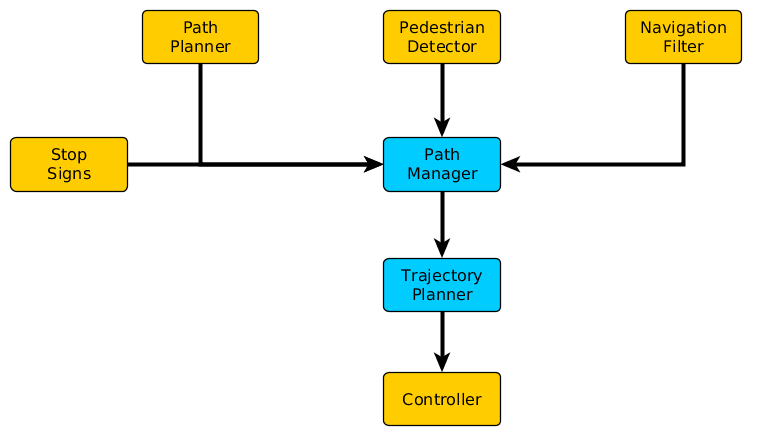
\includegraphics[width=1.0\columnwidth]{graphics/MissingReactionPiece2.png}
  \caption{
    Adding reactive behavior to trajectory planning.
    \newline
    \textbf{!!!!!!!!!!!!!!!!!!!!!!REDO THIS!!!!!!!!!!!!!!!!!!}
  }
  \label{fig:addreact}
\end{figure}

For human passengers, it is widely believed that high levels of jerk (time derivative of acceleration) and high acceleration/velocity values are prime contributors to ride discomfort.
A lot of work has been performed on optimizing these constraints for highways and country roads ~\cite{ziegler14,bahram15,xu12,CHEB15CI}.
Some preliminary work on optimizing these constraints on urban roads has been done ~\cite{Rastelli14,Li15} but they do not consider reactive behavior such as responding to pedestrians or other dynamic objects in the scene.
On the other hand, many systems in the literature which find and plan paths around pedestrians, stop for them, or produce a warning ~\cite{pradalier05,benenson06,gu14,mogelmose15,johnson13} do not work as part of an integrated system that can navigate urban roads.
In this paper, we describe an trajectory generation system that satisfies these constraints for human comfort as well as reactive to presence of pedestrians on the road.

% tracking
Once a trajectory plan is formulated, it must be utilized online in order for a reference signal to be sent to the controllers which govern steering, braking, and engine speed.
This is the trajectory tracking problem, which is discussed in Section \ref{sec:trajectorytracking}.

%%%%%%%%%%%%%%%%%%%%%%%%%%%%%%%%%%%%%%%%%%%%%%%%%%%%%%%%%%%%%%%%%%%%%%%%%%%%%%%%
%%%%%%%%%%%%%%%%%%%%%%%%%%%%%%%%%%%%%%%%%%%%%%%%%%%%%%%%%%%%%%%%%%%%%%%%%%%%%%%%

\section{Input Subsystems} \label{sec:inputsubsystems}

We assume that we have access to Path Planner. This can be for example a service similar to
Google Maps except that it provides lane level maps. We also assume that we have a High
Resolution digital map with Lane centers, Stop signs, crosswalk geometry, and Turning 
curves at intersections. The starting position the 
car is determined via high grade GPS. The destination is manually input into the system.
Using the path planner, we obtain a path along lane centers from start to the destination.
This plan is output as waypoints, with the waypoints corresponding to stop signs marked.

\begin{figure}[thpb]
  \centering
  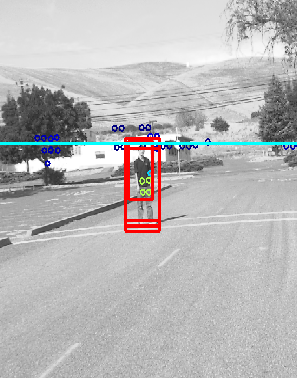
\includegraphics[width=0.5\columnwidth]{graphics/ped2.png}
  \caption{Showing detected pedestrian by the computer vision system
  \newline
  \textbf{!!!!!!!!Crop to save space!!!!!!!!!!!!!!!}
  }
  \label{fig:ped}
\end{figure}

%\begin{figure}[thpb]
%  \centering
%  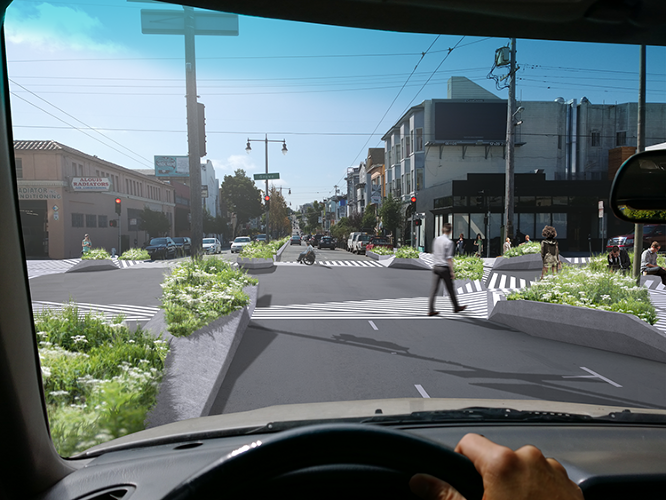
\includegraphics[width=1.0\columnwidth]{graphics/3023096-slide-c4carafter.png}
%  \caption{Pedestrain at the intersection}
%  \label{fig:ped2}
%\end{figure}

\begin{figure}[thpb]
  \centering
  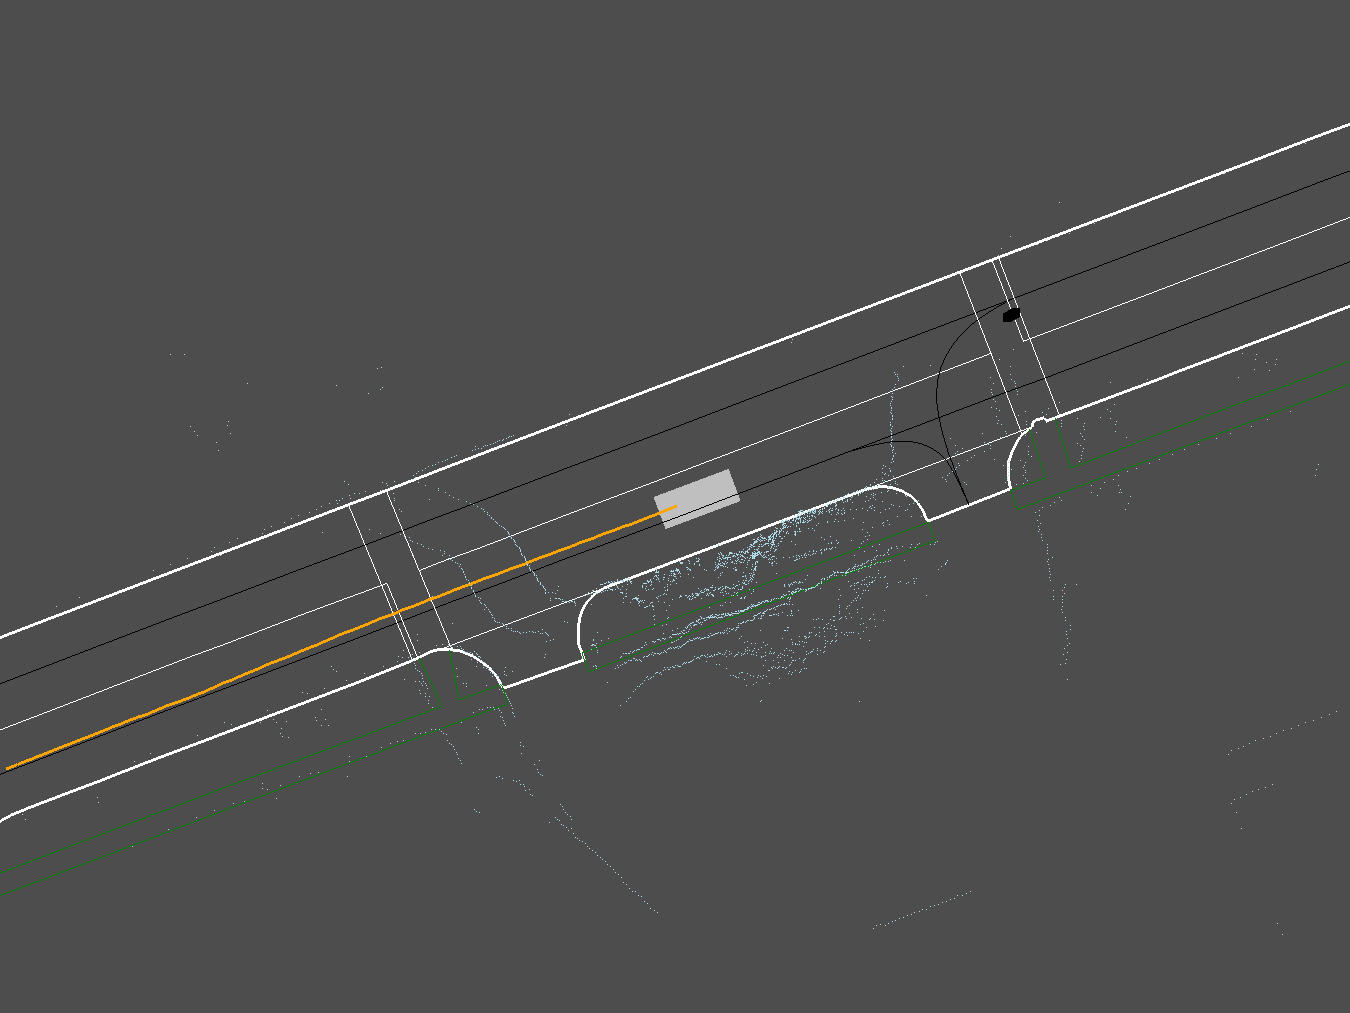
\includegraphics[width=1.0\columnwidth]{graphics/screenshot-objectmap.png}
  \caption{Showing car with road and path covered so far. The red filled circle shows the pedestrian for which the car is stopping}
  \label{fig:car}
\end{figure}

Pedestrian Detection is performed via a Camera, and LiDAR system. It computes a bounding 
box for each pedestrian as shown in Figure \ref{fig:ped}. The pedestrian position is 
transformed to the vehicle body frame, and subsequently transformed to global frame and 
can be shown on the map as in Figure \ref{fig:car}.

\begin{figure}[thpb]
  \centering
  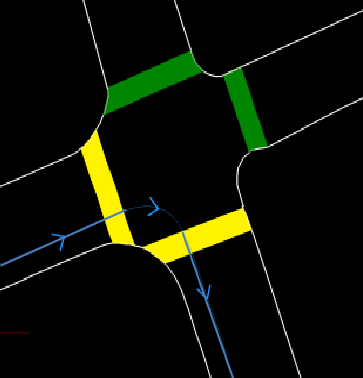
\includegraphics[width=0.5\columnwidth]{graphics/IntersectionCrosswalks.png}
  \caption{A car turning right at the intersection only needs to care about pedestrians in the 
pedestrian crossings shown yellow. Pedestrians in the green crossings can be ignored unless they
appear somewhere on the road}
  \label{fig:intersect}
\end{figure}

We also have an In-Out Algorithm implemented via polygon intersection that can be used to
ignore “safe” pedestrians that are on sidewalks, off-path crosswalks, and behind planned stop
as shown in Figure \ref{fig:intersect}.
Remaining pedestrians pose collision risk and we need to reactively slow down or stop for them.
This is accomplished by sending stop message with pedestrian locations to path manager.

For Navigation Filtering we use an ADMA-G based Commercial automotive GPS/INS system.
It receives RTK corrections via cell modem. It outputs Global position, global heading,
body frame velocity and body frame acceleration to 10s of cms.

%%%%%%%%%%%%%%%%%%%%%%%%%%%%%%%%%%%%%%%%%%%%%%%%%%%%%%%%%%%%%%%%%%%%%%%%%%%%%%%%
%%%%%%%%%%%%%%%%%%%%%%%%%%%%%%%%%%%%%%%%%%%%%%%%%%%%%%%%%%%%%%%%%%%%%%%%%%%%%%%%

\section{Trajectory Planning} \label{sec:trajectoryplanning}

For the purposes of this work, the objective of trajectory planning is to take a 2 dimensional (horizontal plane) path, and compute a series of constant jerk intervals for motion along the length of the path which is time optimal yet still falls within constraints on speed, acceleration, and jerk.
Elevation changes will not be addressed here.
Integrating piecewise constant jerk over time yields acceleration which is piecewise linear over time, speed which is piecewise quadratic over time, and position which is piecewise cubic over time.
We assume that the path planner operates independently from the trajectory planner and tracker.
Prescribed initial and end conditions for position, speed, and acceleration must also be honored.
This means that the desired trajectory plan is one dimensional, so using curvilinear coordinates will significantly simplify the solution.
We show how two dimensional concerns (specifically cornering speeds for this work) are expressed in one dimension to guide planning.
All planning is longitudinal; that is, speed is the primary focus, and we assume that a separate yaw controller will ensure that the vehicle follows the prescribed path.

\begin{figure}[thpb]
  \centering
  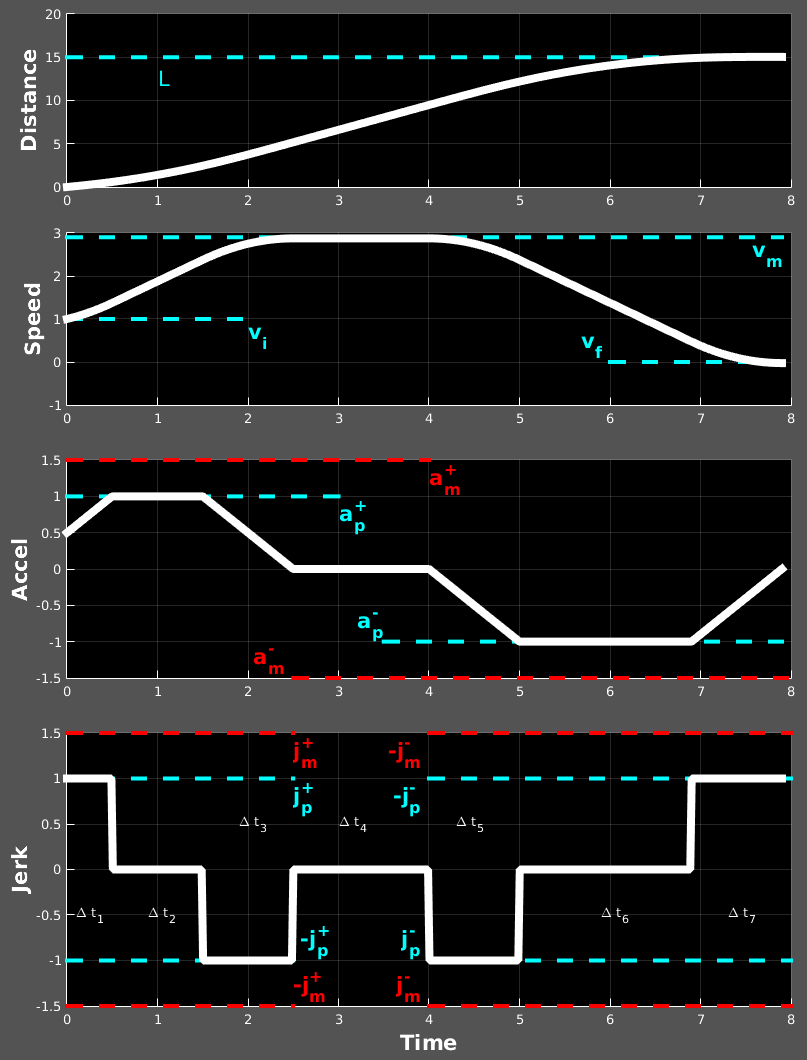
\includegraphics[width=1.0\columnwidth]{graphics/Full7PhaseSpecVertical.png}
  \caption{
    7 phase constant jerk profile along curvilinear distance axis.
    All values needed to completely parameterize a single path segment for trajectory are labelled here.}
  \label{fig:full7phasespec}
\end{figure}

%%%%%%%%%%%%%%%%%%%%%%%%%%%%%%%%%%%%%%%%%%%%%%%%%%%%%%%%%%%%%%%%%%%%%%%%%%%%%%%%

\subsection{Jerk Profiles} \label{sec:jerkprofiles}

Consider, as a starting point, the case in which a vehicle is moving at some small initial speed and needs to accelerate to some travelling speed, maintain that speed for some distance, then brake to a stop at a prescribed end location.
Figure \ref{fig:full7phasespec} shows this trajectory over time.
The problem is defined by the vector of known values $\mathbf{b}  = [v_i, a_i, L, v_m, v_f]$, being initial speed, initial acceleration, the total distance, speed limit, and the final speed, respectively.
It is assume that the final forward acceleration will be zero.
If the magnitude of the desired peak acceleration and jerk ($a_m$ and $j_m$, respectively) are known, then the profile with $M$ jerk phases (7 in this case) can be generated by solving for the time intervals $[\Delta t_1, ..., \Delta t_M]$.
Jerk and peak acceleration may be different when reducing speed versus increasing speed to more closely mirror human driving behavior \emph{Citation}.
The remaining parameters yet to be set now become $\mathbf{a}_m = [a^+_m , a^-_m]$ and $\mathbf{j}_m = [j^+_m , j^-_m]$.
As we will show later, peak acceleration and jerk must sometimes be modified to obtain physically possible time intervals.
To enable this, ranges of acceptable longitudinal jerk and acceleration $\mathbf{a}^{max}_m = [a^{+,max}_m , a^{-,max}_m]$ and $\mathbf{j}^{max}_m = [j^{+,max}_m , j^{-,max}_m]$ are set according to the relation in Eqs. \ref{eq:am} and \ref{eq:jm}.
This is computed for every point along the path.
In the simplest case, one value for each of the quantities expressed in those relations may be chosen for the entire path.

\begin{equation}
  a^{+,max}_m >= a^+_m > 0 > a^-_m >= a^{-,max}_m
  \label{eq:am}
\end{equation}
\begin{equation}
  j^{+,max}_m >= j^+_m > 0 > j^-_m >= j^{-,max}_m
  \label{eq:jm}
\end{equation}

It is obvious that there are many cases in which this solution will fail.
For instance, if $L$ is sufficiently short and $v_m$ is sufficiently high, then it will not be possible to ever reach $v_m$ with realistic values of $\mathbf{a}_m$ and $\mathbf{j}_m$.
We propose that 4 other basic profiles be defined, and an algorithm constructed which judiciously chooses the appropriate profile for every segment defined by a vector $\mathbf{b}$.
The other profiles are explained below in Section \ref{sec:jerkprofiles}.
A path is then a set of $N_s$ segments, each of which is defined by a set of parameters $\mathbf{b}_k, k = 1 ... N_s$ and can be solved indivually in sequence.
Determination of where to break a path into segments is discussed below in Section \ref{sec:pathsegmentation}.

There are a total of five potential jerk profiles which have been created to cover all feasible values in $\mathbf{b}$.
All impossible scenarios are automatically ruled out (e.g., end speed above speed limit, travelling speed of zero, negative speeds in $\mathbf{b}$, etc).
It should be noted that travelling backward (i.e., in reverse gear) is not supported in this work.
To find closed-form solutions for each, a symbolic solver was used.
The target values for each profile are the time steps between jerk changes.
These are solved by plugging in $\mathbf{b}$, $\mathbf{a}_m$, and $\mathbf{j}_m$.

For each of the profiles, it is possible that the chosen values of $\mathbf{a}_m$ and $\mathbf{j}_m$ will not be feasible for a desired speed at the end of the phase.
This results in a negative time interval for that phase.
In many cases, modifying $\mathbf{a}_m$ and $\mathbf{j}_m$ such that they still lie within $\mathbf{a}^{max}_m$ and $\mathbf{j}^{max}_m$ will remedy this.
Specifically, jerk may be increased while peak acceleration is decreased.
This process is referred to herein as ``accel-jerk tuning''
If no acceptable values are found within the valid ranges of $\mathbf{a}^{max}_m$ and $\mathbf{j}^{max}_m$, a new jerk profile must be chosen.

To decide which profile to employ, a cascade approach is used.
Analytic values of time intervals are evaluated for each profile by plugging in values of $\mathbf{b}$, $\mathbf{a}_m$, and $\mathbf{j}_m$ until all time intervals are positive and real.
The order in which they are attempted is: 7 $\rightarrow$ 6 $\rightarrow$ 4 $\rightarrow$ 4R $\rightarrow$ 3.

\subsubsection{7 Phase} \label{sec:7phase}

This profile, described above, is always attempted first.
All time steps have a single solution, enabled by the fact that the initial and end conditions are known, and the two peak accelerations and two jerk magnitudes are provided as configuration parameters.
In the case where $\Delta t_2$ or $\Delta t_6$ are negative, accel-jerk tuning must be employed.
In the instance where $\Delta t_4$ is negative, the total segment length $L$ is too short to reach top speed of $v_m$, so a 6 phase profile must be used.

\subsubsection{6 Phase} \label{sec:6phase}

In the case mentioned above, the speed limit is too high for a solution to exist for a 7 phase profile.
The middle travel period $\Delta t_4$ is removed, so that the vehicle increases speed and then immediately decreases speed. 
The peak speed in this case has a solution, but cannot be manipulated directly.
Without this known value, the problem becomes underdefined, so $\Delta t_2$ and $\Delta t_5$ each have two solutions: one negative and one positive.
The positive solution is chosen.
In the case where both solutions are negative, accel-jerk tuning is attempted. 
Should that yield no positive time intervals, one of the two 4 phase profiles then becomes appropriate, since $L$ is not large enough to accomodate accelerating past the end speed.
If $v_i > v_f$, then a reversed 4 phase profile is attempted.
However, if $v_i > v_f$, then a regular 4 phase profile is attempted.

\begin{figure}[thpb]
  \centering
  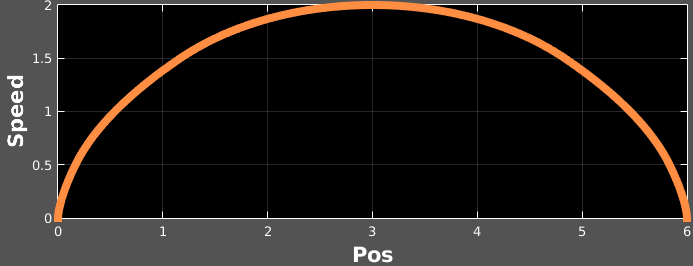
\includegraphics[width=0.7\columnwidth]{graphics/6phase_v(s).png}
  \caption{6 phase profile, displayed as speed vs. position along path}
  \label{fig:6phaseprofile}
\end{figure}

\subsubsection{4 Phase} \label{sec:4phase}

When $v_i < v_m \simeq v_f$, the vehicle should increase speed, then maintain that speed for the distance remaining in the segment.

\begin{figure}[thpb]
  \centering
  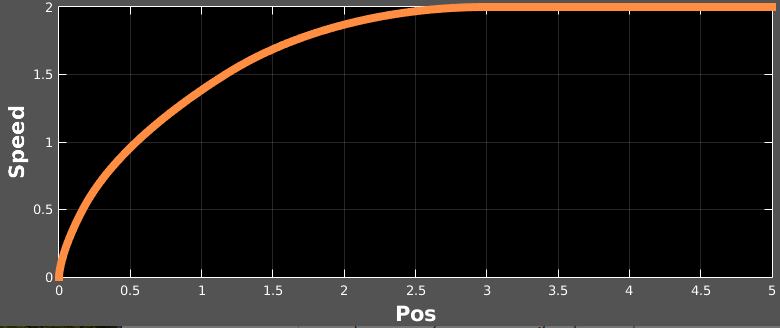
\includegraphics[width=0.7\columnwidth]{graphics/4phase_v(s).png}
  \caption{4 phase profile, displayed as speed vs. position along path within the segment.}
  \label{fig:4phaseprofile}
\end{figure}

\subsubsection{Reversed 4 Phase} \label{sec:reversed4phase}

When $v_i \simeq v_m > v_f$, it would be nonsensical to immediately brake.
The initial speed is maintained for a period before applying the brakes.

\begin{figure}[thpb]
  \centering
  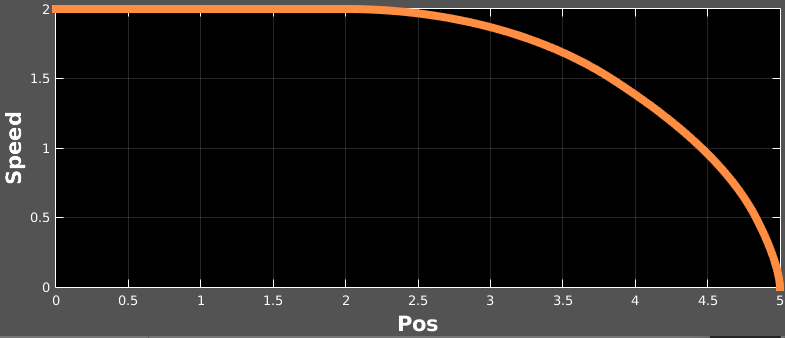
\includegraphics[width=0.7\columnwidth]{graphics/4Rphase_all_derivatives.png}
  \caption{Reversed 4 phase profile, displayed as speed vs. position along path within the segment.}
  \label{fig:4rphaseprofile}
\end{figure}

\subsubsection{3 Phase} \label{sec:3phase}

A change from one speed to another.
All of the above profiles are composed of some combination of a 3 phase profile and a $j_k = 0$ phase.
This presents a difficulty in that either $L$ or $v_f$ may be enforced, but not both (there is no solution to enforce both).
As such, this profile is chosen only for a segment in which it is impossible to completely arrive at the end speed given the initial speed, so fitting one of the two 4 phase profiles has been attempted and subsequently failed.

\begin{figure}[thpb]
  \centering
  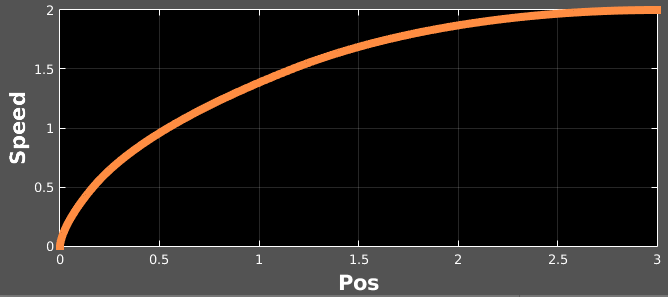
\includegraphics[width=0.7\columnwidth]{graphics/3phase_v(s).png}
  \caption{3 phase profile, displayed as speed vs. position along path.}
  \label{fig:3phaseprofile}
\end{figure}

%%%%%%%%%%%%%%%%%%%%%%%%%%%%%%%%%%%%%%%%%%%%%%%%%%%%%%%%%%%%%%%%%%%%%%%%%%%%%%%%

\subsection{Path Segmentation} \label{sec:pathsegmentation}

% make sure to incorporate extensibility to other constraints
The goal of the segmentation process is to divide a given path into multiple portions where each has a uniform upper limit on speed, acceleration, and braking.
There are 3 steps in the segmentation process:
\begin{enumerate} \label{asdf}
  \item \emph{Ceiling calculation}, where $\mathbf{b}$, $\mathbf{a}_m$, and $\mathbf{j}_m$ are found for every point in the given path.
  \item \emph{Clustering}, in which path points are grouped sequentially.
  \item \emph{Consolidation}, in which a single $\mathbf{b}$, $\mathbf{a}_m$, and $\mathbf{j}_m$ is selected for each segment.
\end{enumerate}
After this is done, the process described above in Section \ref{sec:jerkprofiles} may be applied to each of the segments.

The ceiling calculation is a minimax problem.
Each of the 9 scalars is a minimum of several maxima computed from an arbitrary set of constraints.
For instance, acceleration constraints may include a set of limits derived from friction coefficients at every point along the path.

% How we actually did this.
For the purposes of developing a simple example application, two constraints will be used for $v_{m,k}$: legal speed limit ($SL$, set constant for the whole path) and lateral acceleration limit ($a_{B,y}^{max}$. 
Lateral acceleration constraints are translated into longitudinal speed constraints using the approximation $v_{m,k}(a_{B,y}) = \sqrt{a_{B,y}^{max}/\kappa_k}$ for $k = 1, ..., N_p$.
For each path point, the value $v_{m,k}(a_{B,y}^{max})$ denotes the speed necessary to obtain the limit lateral acceleration, denoted by $a^{max}_{B,y}$.
The value $\kappa_k$ denotes the path curvature at each point.

This information is used to choose the segment boundaries in the clustering step.
Any number of clustering algorithms may be used here, and prudent choice of segment boundaries is arguably one of the most critical pieces of trajectory planning process.
For the present example, we will choose a simple univariate heuristic which essentially identifies curves in the roadway.
Each time that $v_{m,k} < SL$ becomes true, a curve is beginning, and a segment boundary is drawn.
Each time that $v_{m,k} = SL$ is once again true, the current curve has ended, and another segment boundary is drawn.
Figure \ref{fig:course_highlight_turns} shows the result of this algorithm. 

\begin{figure}[thpb]
  \centering
  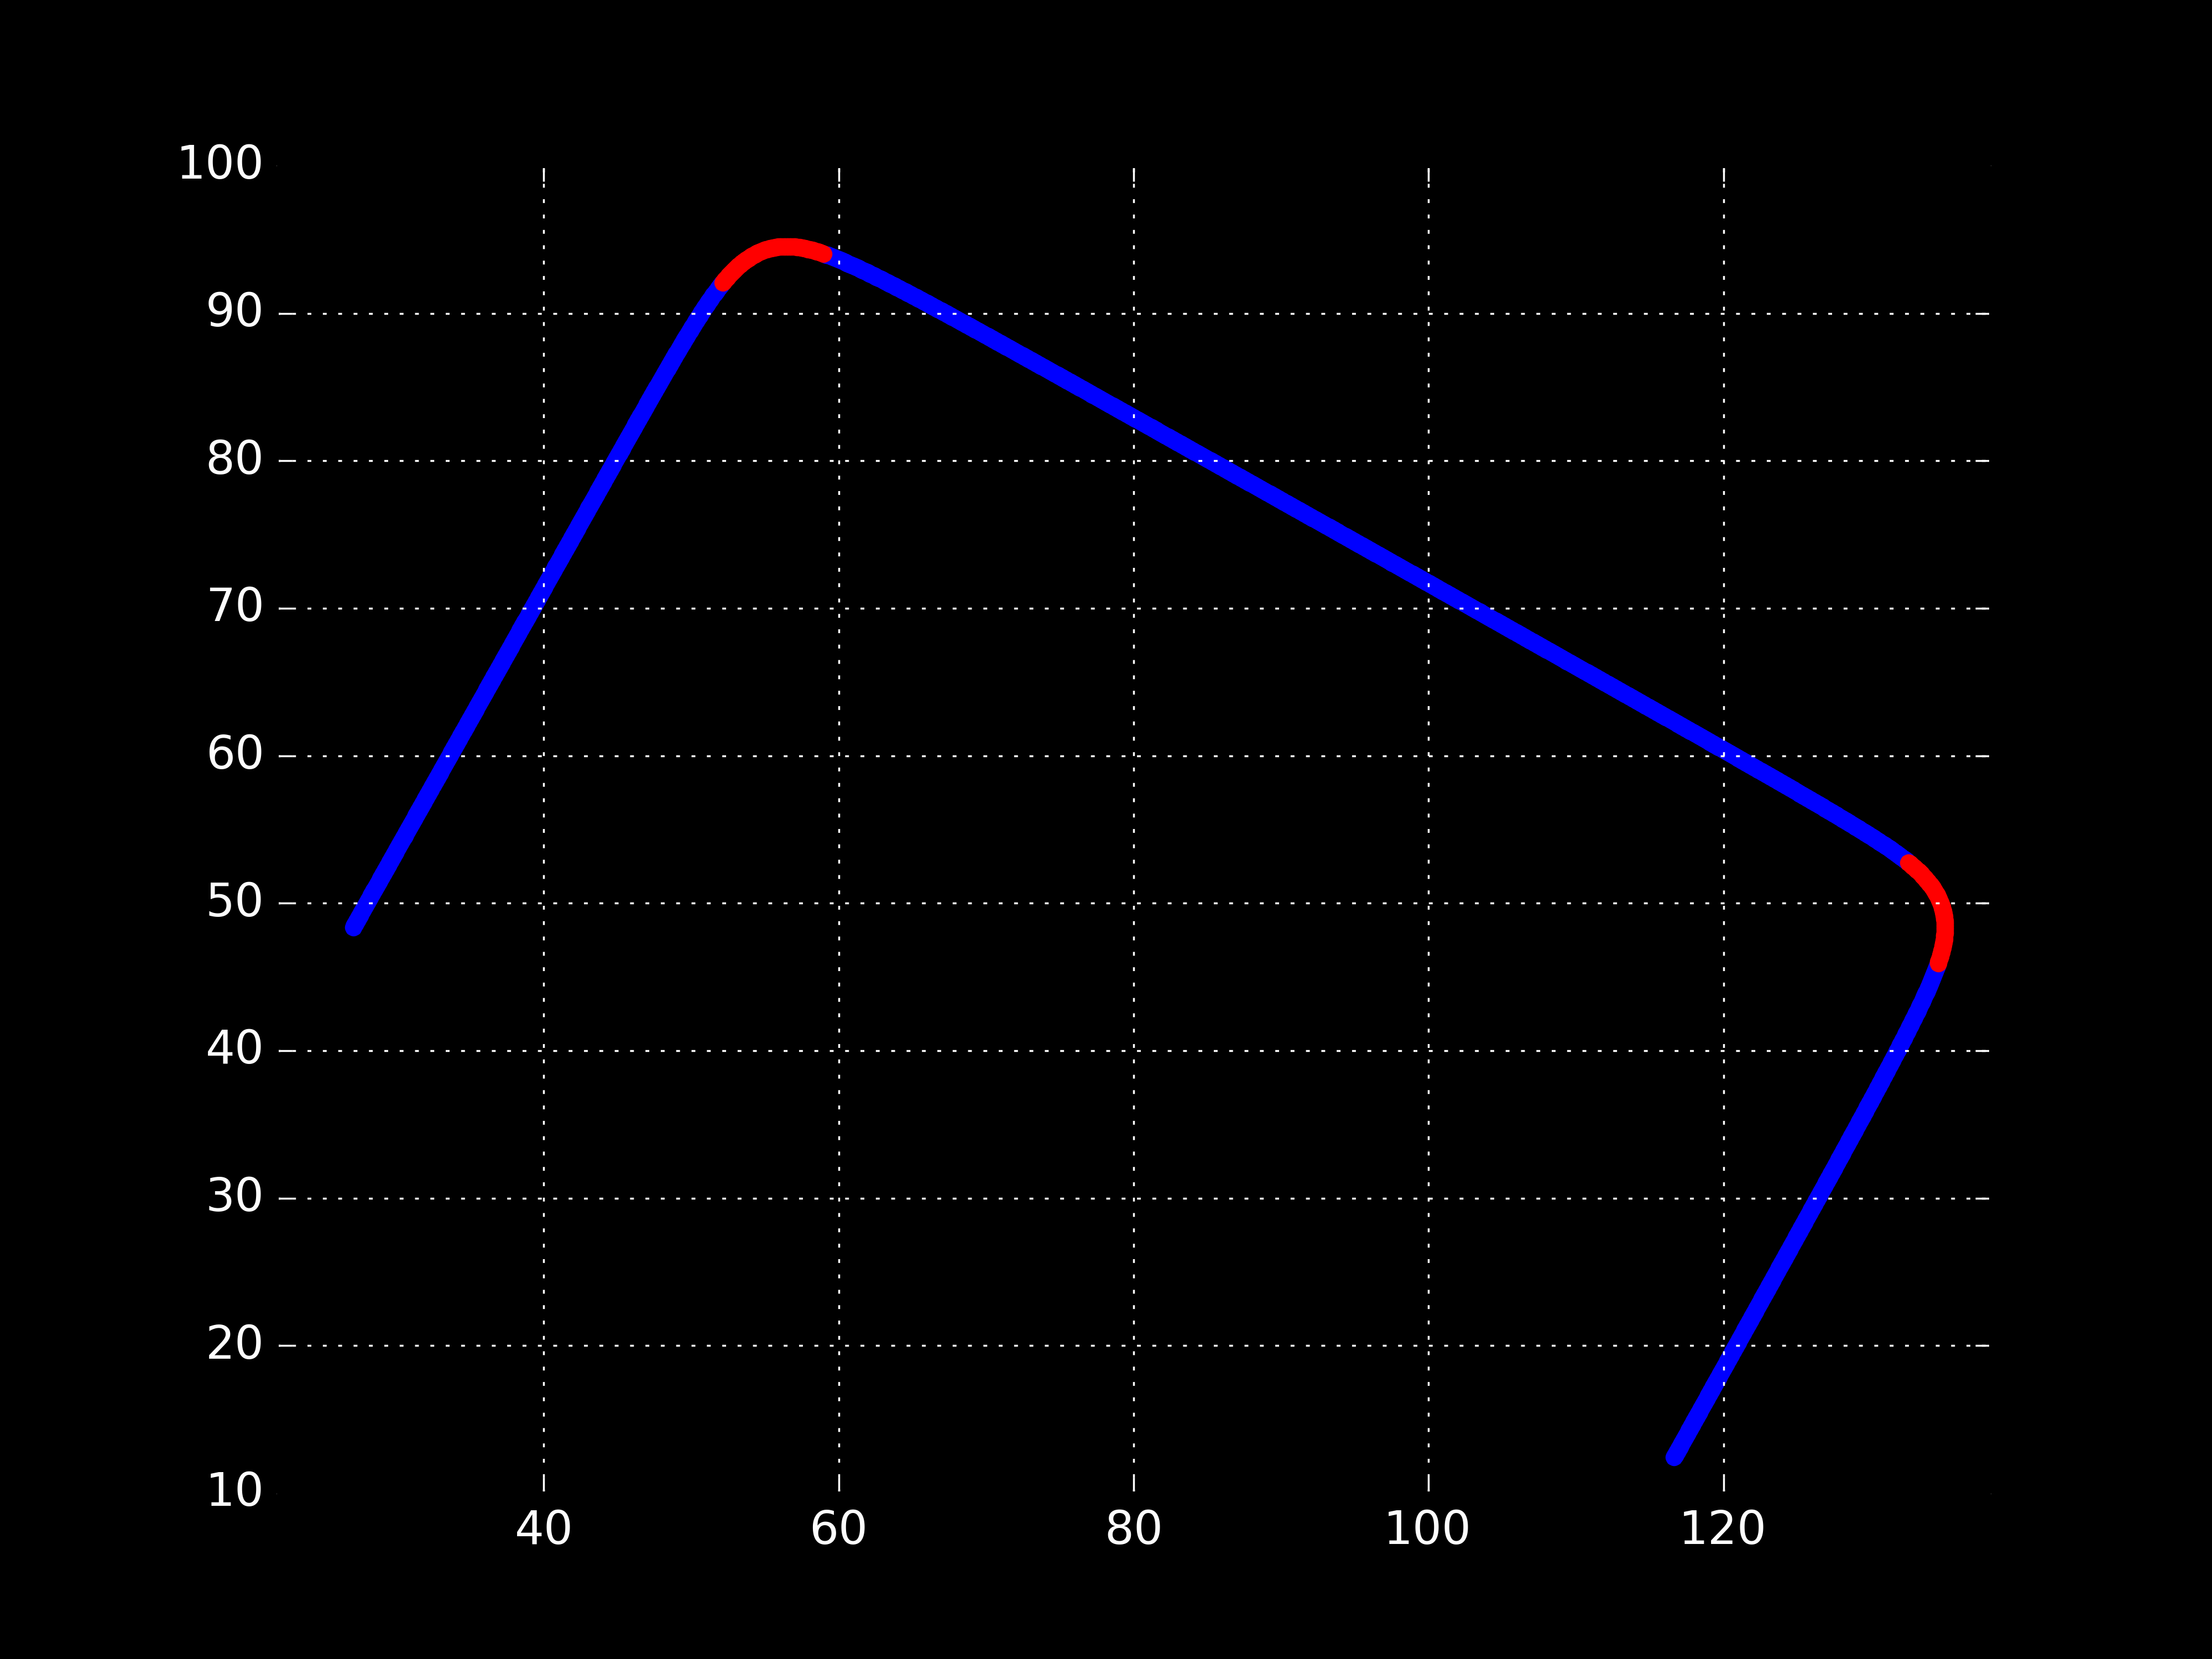
\includegraphics[width=0.8\columnwidth]{graphics/course_highlighted_turns.png}
  \caption{
    Clustering output for a short path when using an algorithm which draws segment boundaries around curves.
    Portions in red indicate areas where the longitudinal speed required to adhere to lateral acceleration limits is below the legal speed limit of 11.176 m/s (25 mi/hr).
  }
  \label{fig:course_highlight_turns}
\end{figure}

% need better notation here.
In the consolidation step, a single set of $\mathbf{g}$, $\mathbf{a}_m$, and $\mathbf{j}_m$ must be calculated for each segment using the values corresponding to each of the path points which comprise the segment in question.
The minimum of scalar across all constituent points is chosen.
While not time optimal, it does ensure that no constraints are violated while still keeping the number of total segments low.
In the present example, this means that in the straight portions of the path $v_m = SL$ and in the curves $v_m$ is set to the value required to obtain $a_{B,y}^{max}$ for the entireity of the curve.
As a result, many of the curves will have a constant speed.
For the sake of simplicity, the values of $a^+_{m,k}$, $a^-_{m,k}$, $j^+_{m,k}$, and $j^-_{m,k}$ are all set constant for the entire path, using values from \cite{Maurya2012,Hoberock1977,Long2000}.

\begin{figure}[thpb]
  \centering
  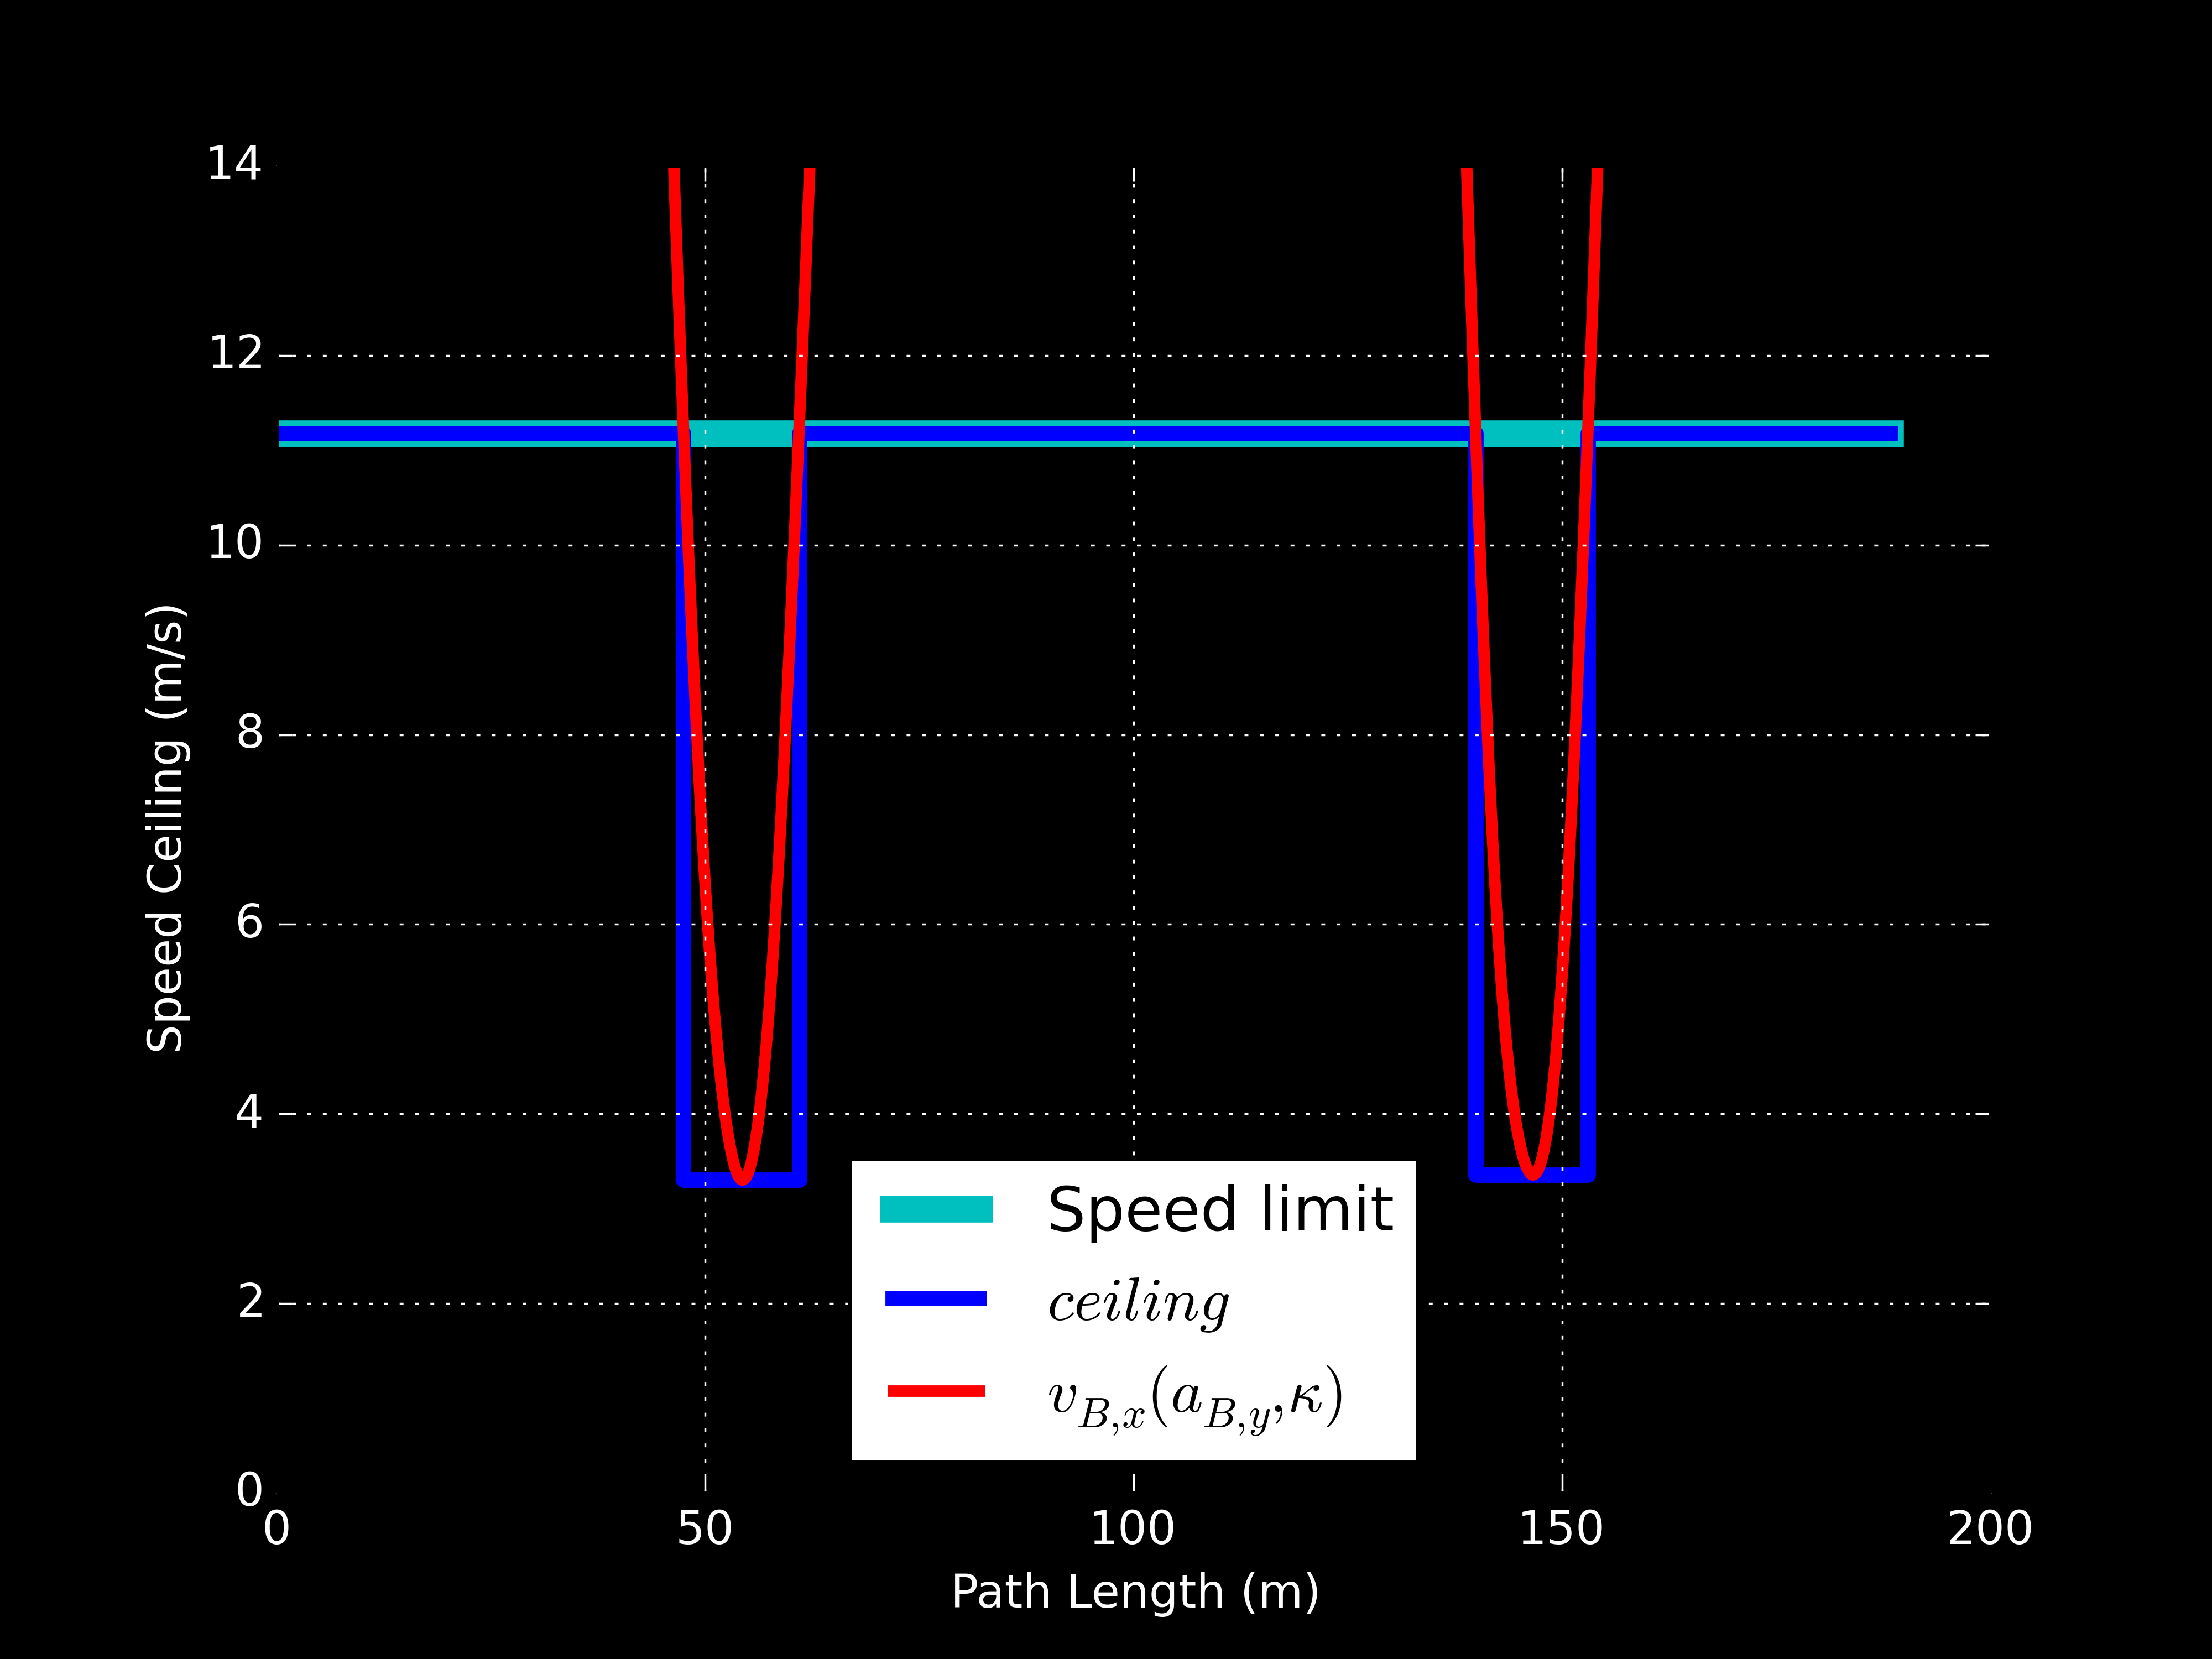
\includegraphics[width=0.8\columnwidth]{graphics/speed_ceiling.png}
  \caption{
    Example of $v_m$ consolidation for simple univariate path clustering which corresponds the the path shown in Figure \ref{fig:course_highlight_turns}.
    The legal speed limit of 11.176 m/s (25 mi/hr) is shown in cyan.
    The longitudinal speed required to adhere to lateral acceleration limits is shown in red.
    The resultant speed ceiling is shown in blue.
  }
  \label{fig:consolidation_speed_ceiling}
\end{figure}

The power of this algorithm is that any set and number of constraints may be used ... \emph{etc., etc., ...}\tabularnewline

%%%%%%%%%%%%%%%%%%%%%%%%%%%%%%%%%%%%%%%%%%%%%%%%%%%%%%%%%%%%%%%%%%%%%%%%%%%%%%%%

\subsection{Unified Solution} \label{sec:unifiedsolution}

At this point, the path has been divided into segments and conditions have been computed such that an analytically derived plan can be fit to each segment individually.
Now a reference trajectory must be generated for the entire path.
Continuity of position, speed, and acceleration is the primary goal of this process.

A jerk vs. time profile is fit to each segment using the algorithm in Section \ref{sec:jerkprofiles}.
Speed and acceleration must be continuous between each segment, but only the corresponding speed ceilings have been found, so the start and end conditions for each segment must be determined.
The values of $a_i$ and $v_i$ for the first segment is set to be the value which is currently reported from sensor data.
Since the final acceleration is set to zero for all profiles, each subsequent segment may begin with $a_i = 0$.
For the final segment, setting $v_f = 0$ is prudent unless the scenario demands otherwise.
To set boundary speed conditions for the interior segments, Algorithm~\ref{alg:segmentspeedboundaryconditions}

\begin{figure}
  \begin{algorithmic}[1]
    \Procedure{SegmentBoundarySpeeds}{$v_m$}
      \State $\mathbf{v}_p \gets \mathbf{v}_m$ \Comment{Initialize targets as ceilings}
      \State $\mathbf{v}_{p,0} \gets v_i$ \Comment{Set starting speed to current}
      \State $\mathbf{v}_p = [\mathbf{v}_p, 0]$ \Comment{Add final speed of 0}
      \For{$k = 1, ..., N_s-1$}
        \If{$v_{m,i+1} > v_{m,i}$}
          \State $v_{p,i+1} \gets v_{m,i}$
        \ElsIf{$v_{m,i+1} > v_{m,i}$}
          \State $v_{p,i+1} \gets v_{m,i+1}$
        \Else
          \State $v_{p,i+1} \gets v_{m,i}$
        \EndIf
      \EndFor
    \EndProcedure
  \end{algorithmic}
\caption{Algorithm to set speed boundary conditions for interior path segments}
\label{alg:segmentspeedboundaryconditions}
\end{figure}

% talk about control points
Now each segment is solved individually.
In the case where a segment requires a speed change which is infeasible given limits on acceleration and jerk, then the final speed for that segment is planned to be the closes possible value.
When these discrepancies in the feasible $v_f$ for a segment arise, the corresponding value in $v_p$ is updated so that the new conditions may be accounted for in the subsequent segment.

At the end of the process, there will be a set of $N_{cp}$ ``control points''.
A control point is a vector $[t_{ref}, s, v_{B,x}, a_{B,x}, j_{B,x}]$ which describes the longitudinal kinematic state of the target vehicle at the moment of an infinite jounce jerk change.
Fitting a jerk profile to each segment results in control points which must be stitched into the control points for the preceding segments.
While no further information than initial conditions, time durations, and jerk values is needed (simple integration would yield lower derivatives of position), this information is already available since it must be solved for each segment.
This extra information may be used as a redundancy layer to verify that no errors occured.
For each segment with $M$ jerk phases, the following is produced:
\begin{itemize}
  \item $M$ time durations $\Delta t_{ref}$. These must be added to the last time value from the previous segment to translate them into reference time.
  \item $M+1$ values of distance elapsed within the segment $\Delta s$. These must be shifted forward by the last $s$ value from the previous segment to translate them into the 1D path domain. Additionally, the first value must be erased.
  \item $M+1$ values of $v_{B,x}$. The first value is checked against the last value from the previous segment to verify equality, then it is erased. These need no translation.
  \item $M+1$ values of $a_{B,x}$. The first value is checked against the last value from the previous segment to verify equality, then it is erased. These need no translation.
  \item $M$ jerk values, which may be appended directly to the preceding jerk values
\end{itemize}

After stitching together control point vectors for time, position, and its derivatives, all information required to have a trajectory plan is now in place.
Since $j(t)$ is piecewise constant, it may be integrated to determine an instantaneous trajectory at any moment in time.
To aid in this, univariate splines are created with time as the independent variable, using the control points as knots.
Position along the path $s(t)$ takes the form of a cubic Hermite spline, constructed using the speed control points $v_{B,x}(t)$ to set the derivatives.
Speed along the path $v_{B,x}(t)$ takes the form of a quadratic Hermite spline, with the acceleration control points $a_{B,x}(t)$ used to set the derivatives at every knot.
Acceleration $a_{B,x}(t)$ is piecewise linear, so lookup is a trivial matter.
The same applies to $j_{B,x}(t)$, which may be implemented with a simple table.

However, the time at which the trajectory plan must be referenced is not always known.
The solution to this problem is known as trajectory tracking, and will be discussed in the next section.

%%%%%%%%%%%%%%%%%%%%%%%%%%%%%%%%%%%%%%%%%%%%%%%%%%%%%%%%%%%%%%%%%%%%%%%%%%%%%%%%
%%%%%%%%%%%%%%%%%%%%%%%%%%%%%%%%%%%%%%%%%%%%%%%%%%%%%%%%%%%%%%%%%%%%%%%%%%%%%%%%

\section{Trajectory Tracking} \label{sec:trajectorytracking}

After planning has been performed, a reference signal must be regularly supplied to a control system in order for the vehicle to carry out the plan.
This is known as tracking.
The primary difficulty here is that the trajectory plan has been developed in a one dimensional position space using a reference time which will have unknown drift relative to real time.
As such, we must find some way to look up the coordinates of the vehicle within the reference trajectory using information typically available for autonomous cars.
A minimal set of such information would include position, velocity vector, heading, and acceleration in the body frame.
After this, it is assumed that the vehicle controller will need samples of a small window into the future trajectory in order to pilot the vehicle.

The general idea is to project the vehicle's current position onto the path then find the cumulative distance along the path between the start point and the projection point.
This is the 1D location corresponding to the vehicle's current reference time.
Once this reference time is obtained, it may be used to look up position, speed, acceleration, and jerk along the curve of the path over the future time window.
From there it is a matter of simple geometry to transform these values into the coordinate system of the path and, subsequently, any other coordinate system which may be needed.

% \subsection{Path Projection} \label{sec:pathprojection}

Several algorithms exist to find the optimal projection of the target vehicle's present kinematic state (position, velocity, and acceleration vectors) onto the path.
A simple approximation, which works well for the path shown in Figure~\ref{fig:course_highlight_turns} is to perpendicularly project the vehicle's position onto a series of lines running between each pair of adjacent points in the path (this will be referred to as a ``link'').
Projections which lie outside of the link's two constituent path points are snapped to that which is nearest.
The projection which is closest to the vehicle's actual position is then assumed to be the correct path projection $\mathbf{r}_p$.
Any number of modifications can be made using heading, velocity vectors, and previous information to allow this method to be extended to complex paths which overlap or self-intersect.

Choosing an algorithm to obtain the current one dimensional position of the vehicle along the length of the path $s_{veh}$ (i.e., in the same one-dimensional coordinate system that planning was performed) is influenced by the form of the path plan.
Assuming that the path is linear between waypoints reduces computational effort significantly.
So $s_{veh}$ at any epoch is then sum of the link lengths behind it's perpendicular projection$\mathbf{r}_p$.
However, the error in this approximation approaches zero as the spacing between path points approaches zero.
Other, more accurate, approximations which work well include cubic splines, arc splines, and Bezier curves, which have solutions for closest point projection and arc-length calculation~\cite{Wang2002,Wang2003,Schindler2011}.

Now the reference time corresponding to the vehicle's location $t_{veh}$ is needed to $v_{B,x}(t)$, $a_{B,x}(t)$, and $j_{B,x}(t)$.
Additionally, it is also needed to sample $s(t)$ at intervals ahead of the vehicle.
Since it is known that $s(t)$ is piecewise cubic, $t(s)$ may be approximated as cubic if a spline is being constructed from knots which have a very high resolution.
In this case, an $s(t)$ spline has already been created using the control points from the unified planning process described in Section~\ref{sec:unifiedsolution}, and it is now resampled at $\Delta t = 0.01 sec$.
This yields two vectors $s'$ and $t'$ which are then used to create a univariate cubic $t(s)$ spline.
Evaluating the $t(s_{veh})$ then yields the current reference time.

%%%%%%%%%%%%%%%%%%%%%%%%%%%%%%%%%%%%%%%%%%%%%%%%%%%%%%%%%%%%%%%%%%%%%%%%%%%%%%%%
%%%%%%%%%%%%%%%%%%%%%%%%%%%%%%%%%%%%%%%%%%%%%%%%%%%%%%%%%%%%%%%%%%%%%%%%%%%%%%%%

\section{Path Manager} \label{sec:pathmanager}


Path Pre-processor conforms the path to planner assumptions. The Path Manager breaks up the
path at stop signs, decides when to stop, when to go and invokes the trajectory planner
as necessary. 

There are two types of stops - Planned (PSTOP) and Reactive (RSTOP). At reactive stops
to pedestrians, the car may slow down and restart if the pedestrian leaves before the
car comes to a stop; otherwise the car would come to a stop and restarts once the 
pedestrian leaves.

The state of the car is represented by a State Machine as shown in figure \ref{fig:st}

\begin{figure}[thpb]
  \centering
  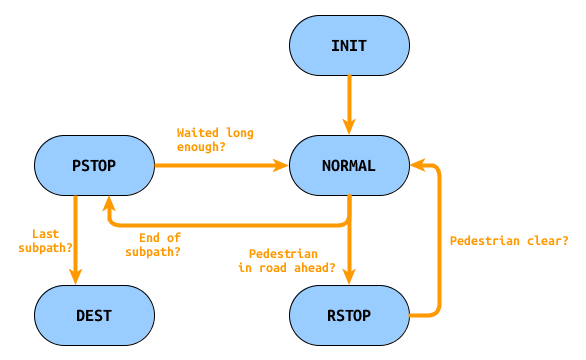
\includegraphics[width=1.0\columnwidth]{graphics/StateMachineSimple.png}
  \caption{State Transition Diagram}
  \label{fig:st}
\end{figure}


The assumption on our work is that there is a unique mapping from a time to s coordinate 
system. This mapping breaks down when we are stopped at a planned or reactive stop. 
The solution is to break the path into sub-paths, and plan and execute incrementally.
This is shown in Figures \ref{fig:segmentation} \ref{fig:stcur} and \ref{fig:scoord}.

\begin{figure}[thpb]
  \centering
  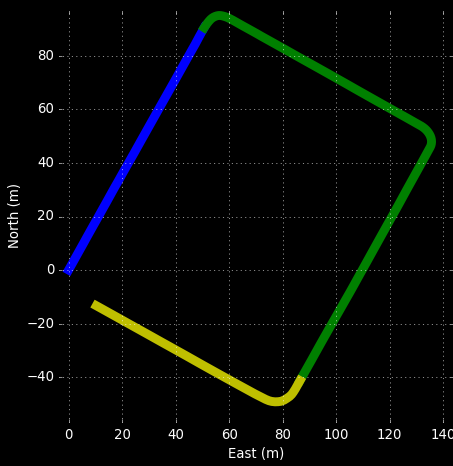
\includegraphics[width=0.5\columnwidth]{graphics/Subpaths.png}
  \caption{Segmentation of the path by path manager. The Trajectory generation is serially called on each segment colored differently. Need to update figure with stop signs????????????????}
  \label{fig:segmentation}
\end{figure}

\begin{figure}[thpb]
  \centering
  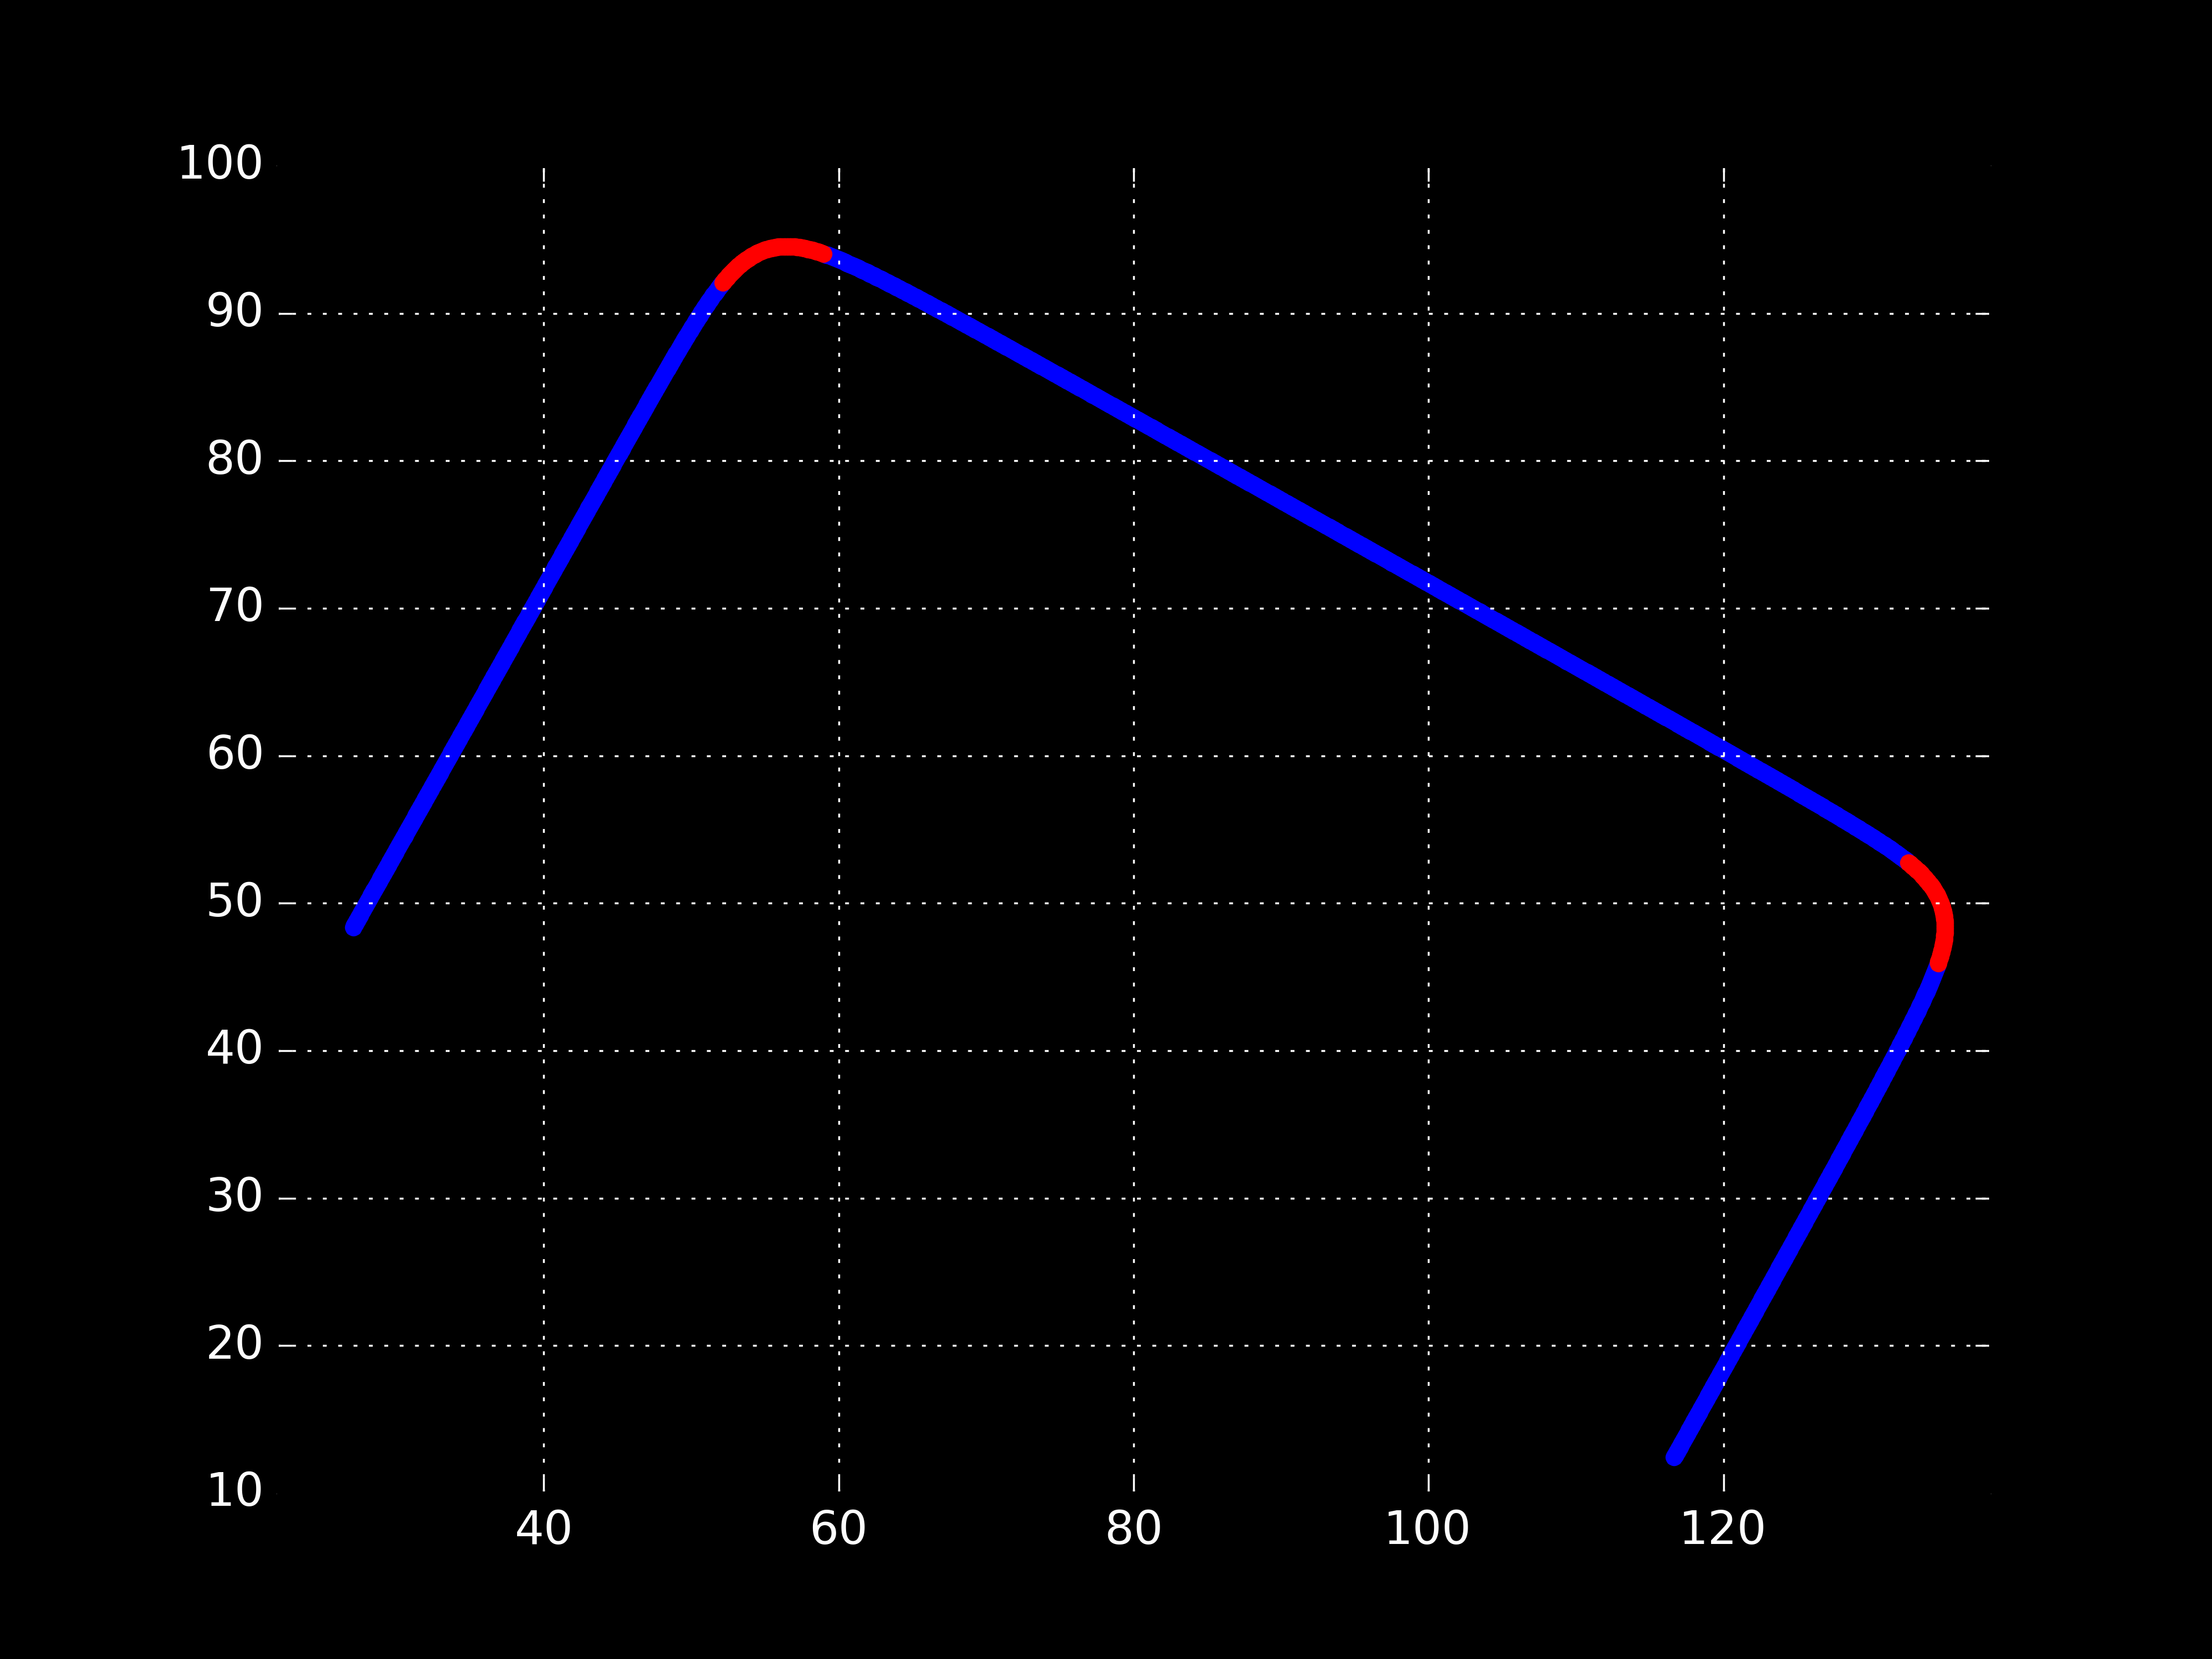
\includegraphics[width=0.5\columnwidth]{graphics/course_highlighted_turns.png}
  \caption{Further characterization of green path shown in segmentation figure into straight and curved parts}
  \label{fig:stcur}
\end{figure}

\begin{figure}[thpb]
  \centering
  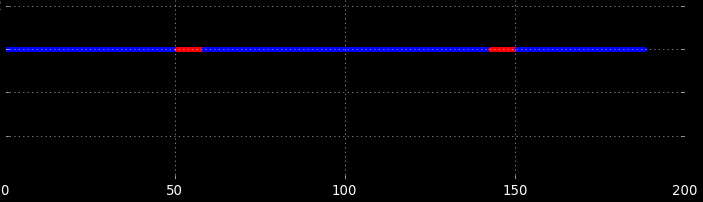
\includegraphics[width=1.0\columnwidth]{graphics/1Dsegmentation.png}
  \caption{Showing the path projected onto the one dimensional s coordinate system}
  \label{fig:scoord}
\end{figure}

The algorithm is:
\begin{itemize}
\item Send first sub-path to trajectory planner
\item Wait until completed
\item Pause for fixed time
\item Send next sub-path to planner
\item Repeat until end of path
\end{itemize}

For unplanned, reactive stops  we need to slow down and stop. There are three scenarios:
\begin{enumerate}
\item Normal pedestrian → appears
\item Stopping pedestrian → moves
\item Stopped pedestrian leaves →
\end{enumerate}

In the next section we describe when/where to begin braking, when/where to stop
and when to go again.

\section{Reactive Subsystem} \label{sec:reactiveubsystem}

\begin{figure}[thpb]
\centering
  \subfigure[Normal mode]{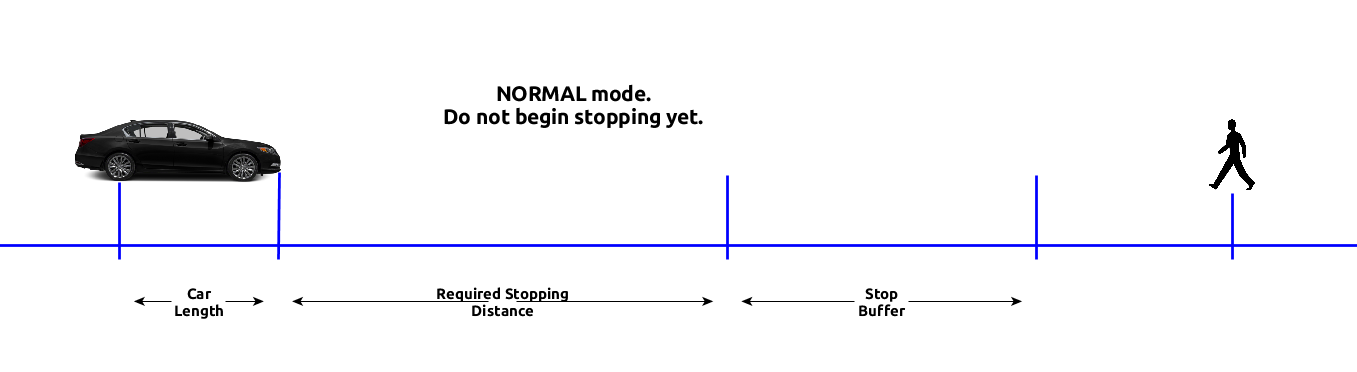
\includegraphics[width=1.0\columnwidth]{graphics/RSTOP_NORMAL.png}}
\\
  \subfigure[Stopping for the pedestrian]{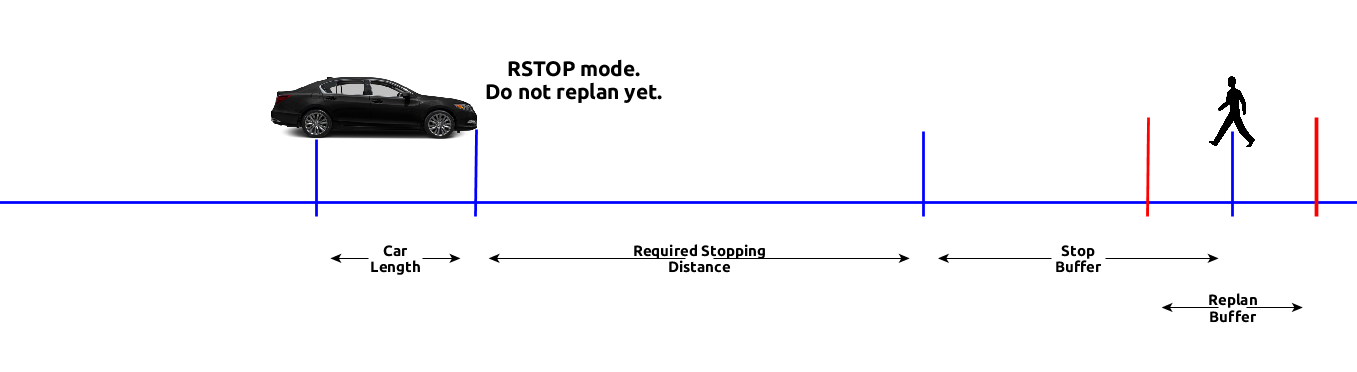
\includegraphics[width=1.0\columnwidth]{graphics/RSTOP_RSTOP.png}}
\\
  \subfigure[Resuming after stop sign]{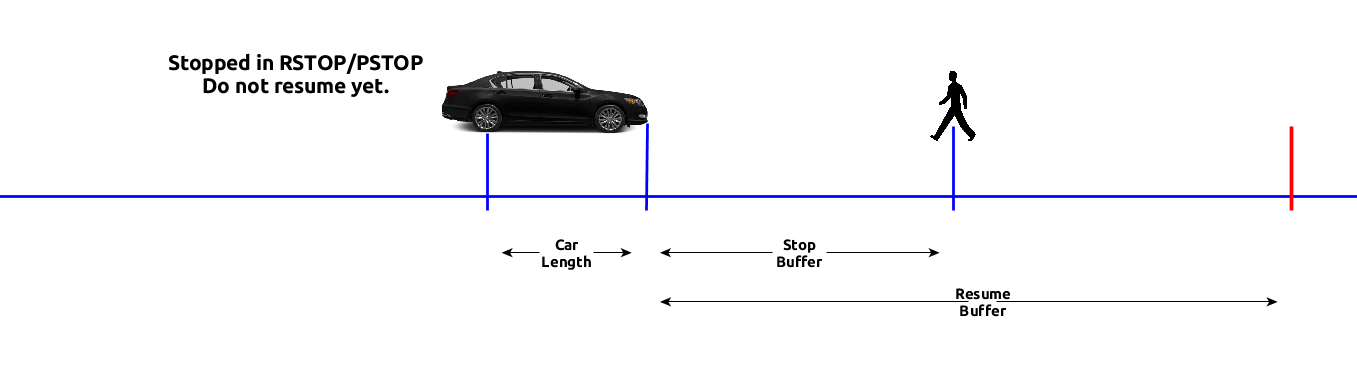
\includegraphics[width=1.0\columnwidth]{graphics/RSTOP_RESUME.png}}
  \caption{Reactive behavior to pedestrain}
  \label{fig:react}
\end{figure}



\begin{figure}[thpb]
  \centering
  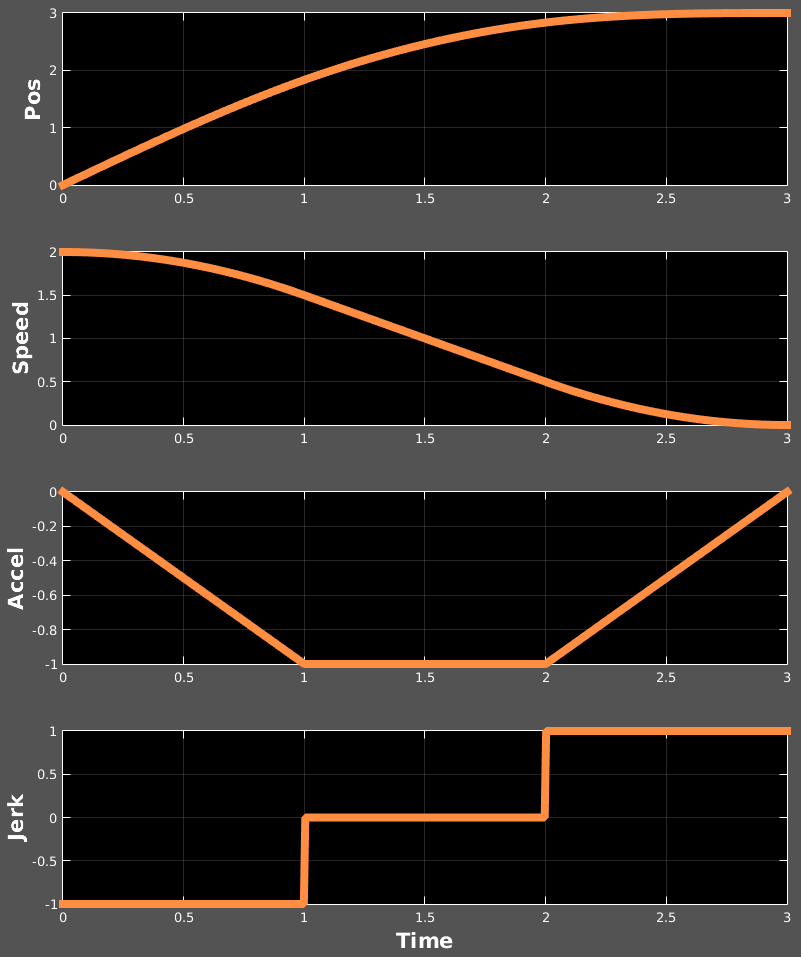
\includegraphics[width=1.0\columnwidth]{graphics/3phase_all_derivatives_SlowingDown.png}
  \caption{3 phase R stop}
  \label{fig:3phaserstop}
\end{figure}


\begin{figure}[thpb]
  \centering
  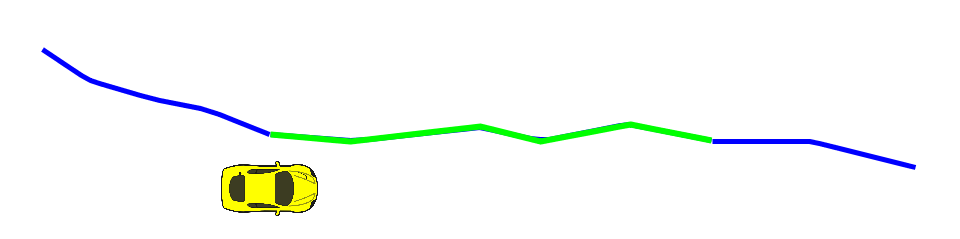
\includegraphics[width=1.0\columnwidth]{graphics/RSTOP_path_truncation.png}
  \caption{Green color path is the one over which the car finds a trajectory to stop}
  \label{fig:pathtostop}
\end{figure}


For reactive stopping, if there are multiple pedestrian ahead, we only consider the
closest pedestrian. That pedestrian is projected on the path of the car to determine the
required braking distance. The stopping trajectory is similar to rest of profile,
and consists of a single segment with 3 phases as shown in Figure \ref{fig:3phase}. 
The trajectory planner uses total distance as parameter, and is not suitable for
our purpose as the end speed constraints are not met. So we reformulate and 
replace $L$ with $v_f$ as hard constraint.

Typically while with the Trajectory Planner, we get initial conditions from the
navigation filter. We use normal (sedate) peak parameters for acceleration
and jerk. We plan a 3 phase stop profile with the current required stopping distance.

Once a pedestrian enters the stop zone, we need to plan, and execute RSTOP trajectory.
When available distance <= “required” distance, we increase acceleration, jerk peaks to
match available distance.

After a reactive stop we split the path before the stop from the one after the stop
sign and execute the later as a separate trajectory. The plan is stored and sampled 
the same as in normal operation.

To get back to normal driving after we are fully stopped, we resume
after pedestrian leaves roadway, or pedestrian moves far down roadway.
When he moved further down, we stop again later after we are a threshold
distance away. The effect is that we follow the person at the distance with some 
delay in chunks of few meters each time. If the pedestrian leaves before 
the car comes to a full stop, the car can speed up without stopping using the 
same algorithm.


\section{Summary} \label{sec:summary}

We have built a robust stopping model as part of Trajectory planner reliably integrated with path manager.
We can travel along desired path, stop at stop signs, stop for pedestrians in roadway, and continue after 
they leave. Our system handles corner cases gracefully, and works with multiple pedestrians as we only 
need to consider the closest pedestrian ahead of us. In future, we want to handle other roadway traffic, 
coexisting with other vehicles. We would also like to perceive and stop for red-lights.

\section{Examples}

\begin{figure}[thpb]
  \centering
  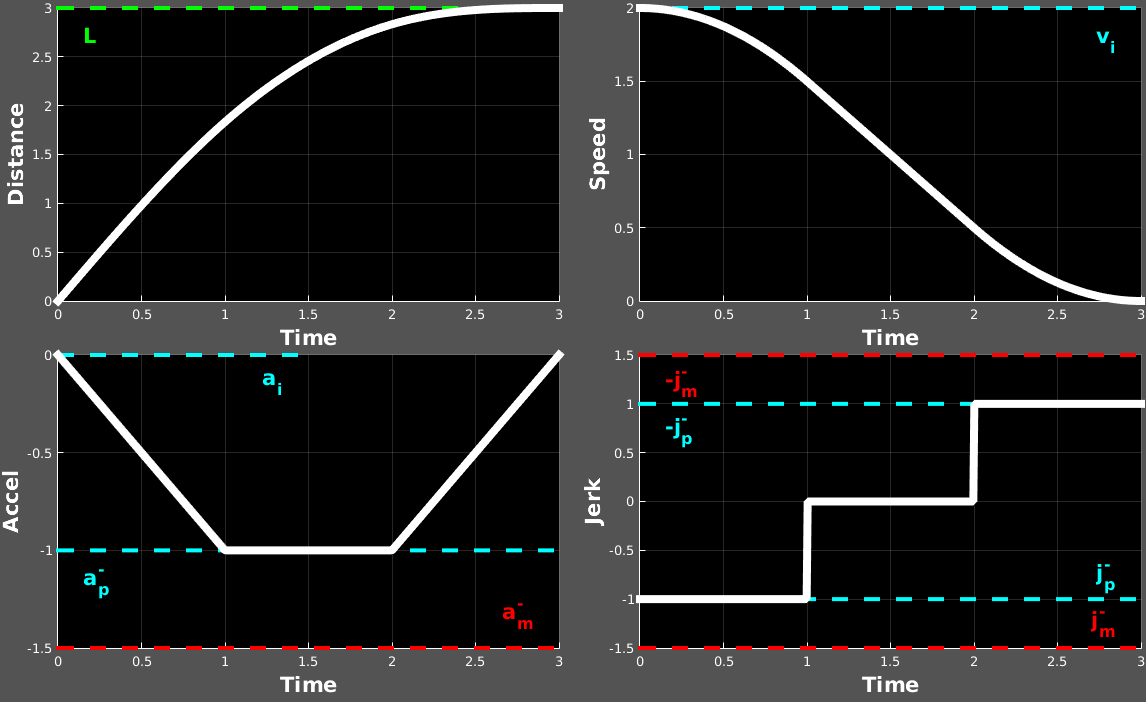
\includegraphics[width=1.0\columnwidth]{graphics/FullStopSpec.png}
  \caption{Example 3 phase jerk profile}
  \label{fig:3phase}
\end{figure}

\section{2d to 1d conversion}


\begin{figure}[thpb]
  \centering
  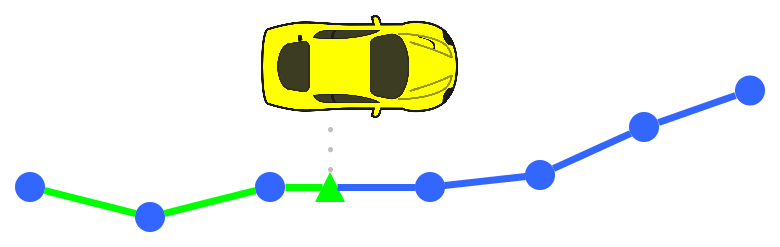
\includegraphics[width=0.5\columnwidth]{graphics/PathProjection.png}
  \caption{Showing projection of current position of car shown by green triangle to s coordinate system}
  \label{fig:cartos}
\end{figure}
\begin{figure}[thpb]
  \centering
  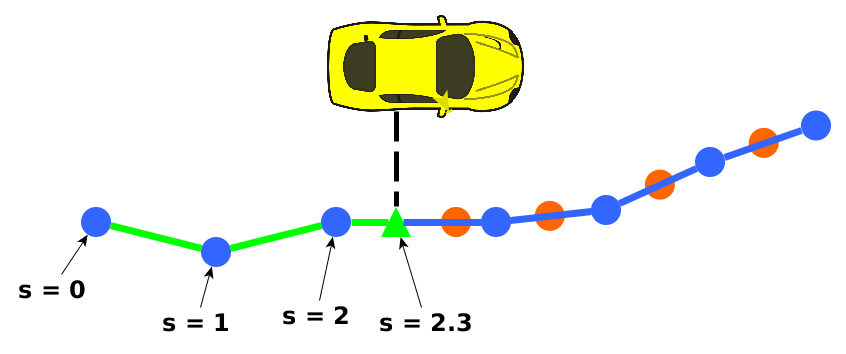
\includegraphics[width=0.5\columnwidth]{graphics/PathProjectionSlice.png}
  \caption{car to s coord with additional points}
  \label{fig:cartos2}
\end{figure}
\begin{figure}[thpb]
  \centering
  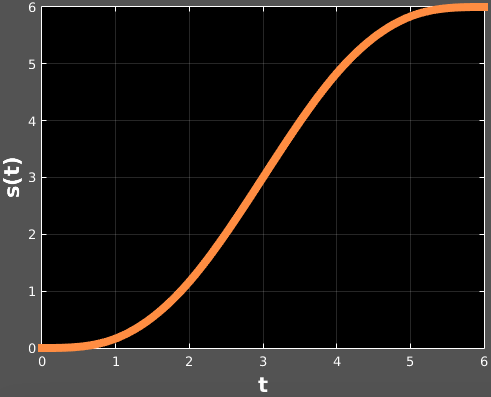
\includegraphics[width=0.5\columnwidth]{graphics/s(t)_generic.png}
  \caption{Transformation from s coordinate system to time}
  \label{fig:stot}
\end{figure}

\section{Other Issues}
                
\begin{figure}[thpb]
  \centering
  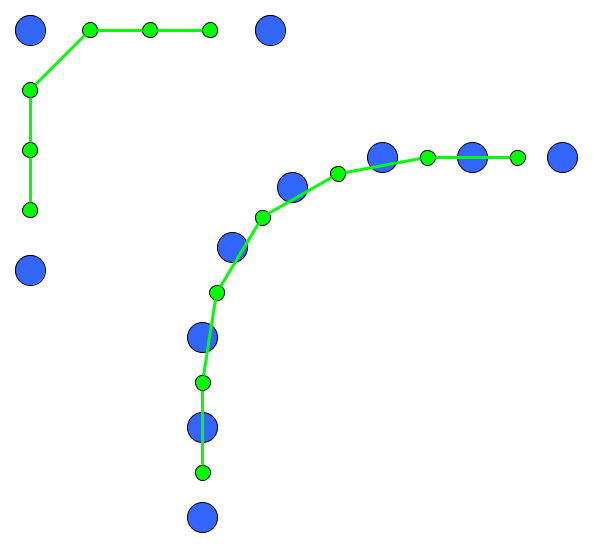
\includegraphics[width=0.5\columnwidth]{graphics/LowResPathSample.png}
  \caption{Grid discretization issue}
  \label{fig:discretization}
\end{figure}
\begin{figure}[thpb]
  \centering
  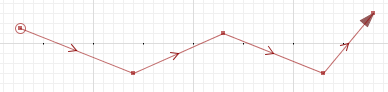
\includegraphics[width=0.5\columnwidth]{graphics/linestring.png}
  \caption{Exaggerated view of path points which may have discontinuous curvature}
  \label{fig:disc}
\end{figure}

\begin{figure}[thpb]
  \centering
  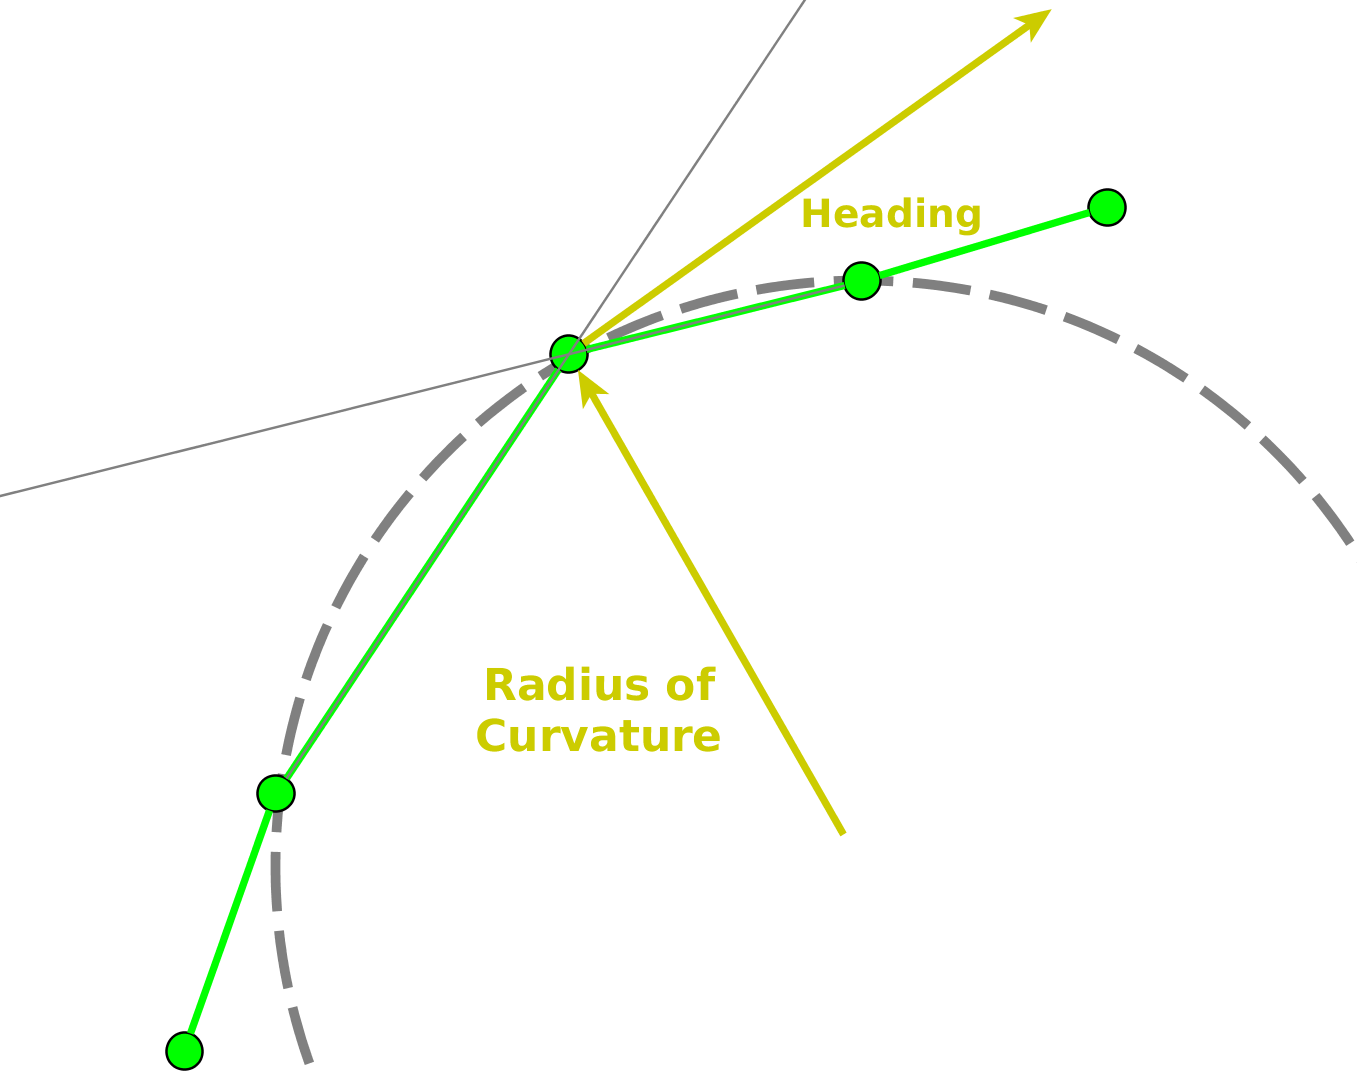
\includegraphics[width=0.5\columnwidth]{graphics/CircularCurvature.png}
  \caption{circular curvature}
  \label{fig:curv}
\end{figure}

\begin{figure}[thpb]
  \centering
  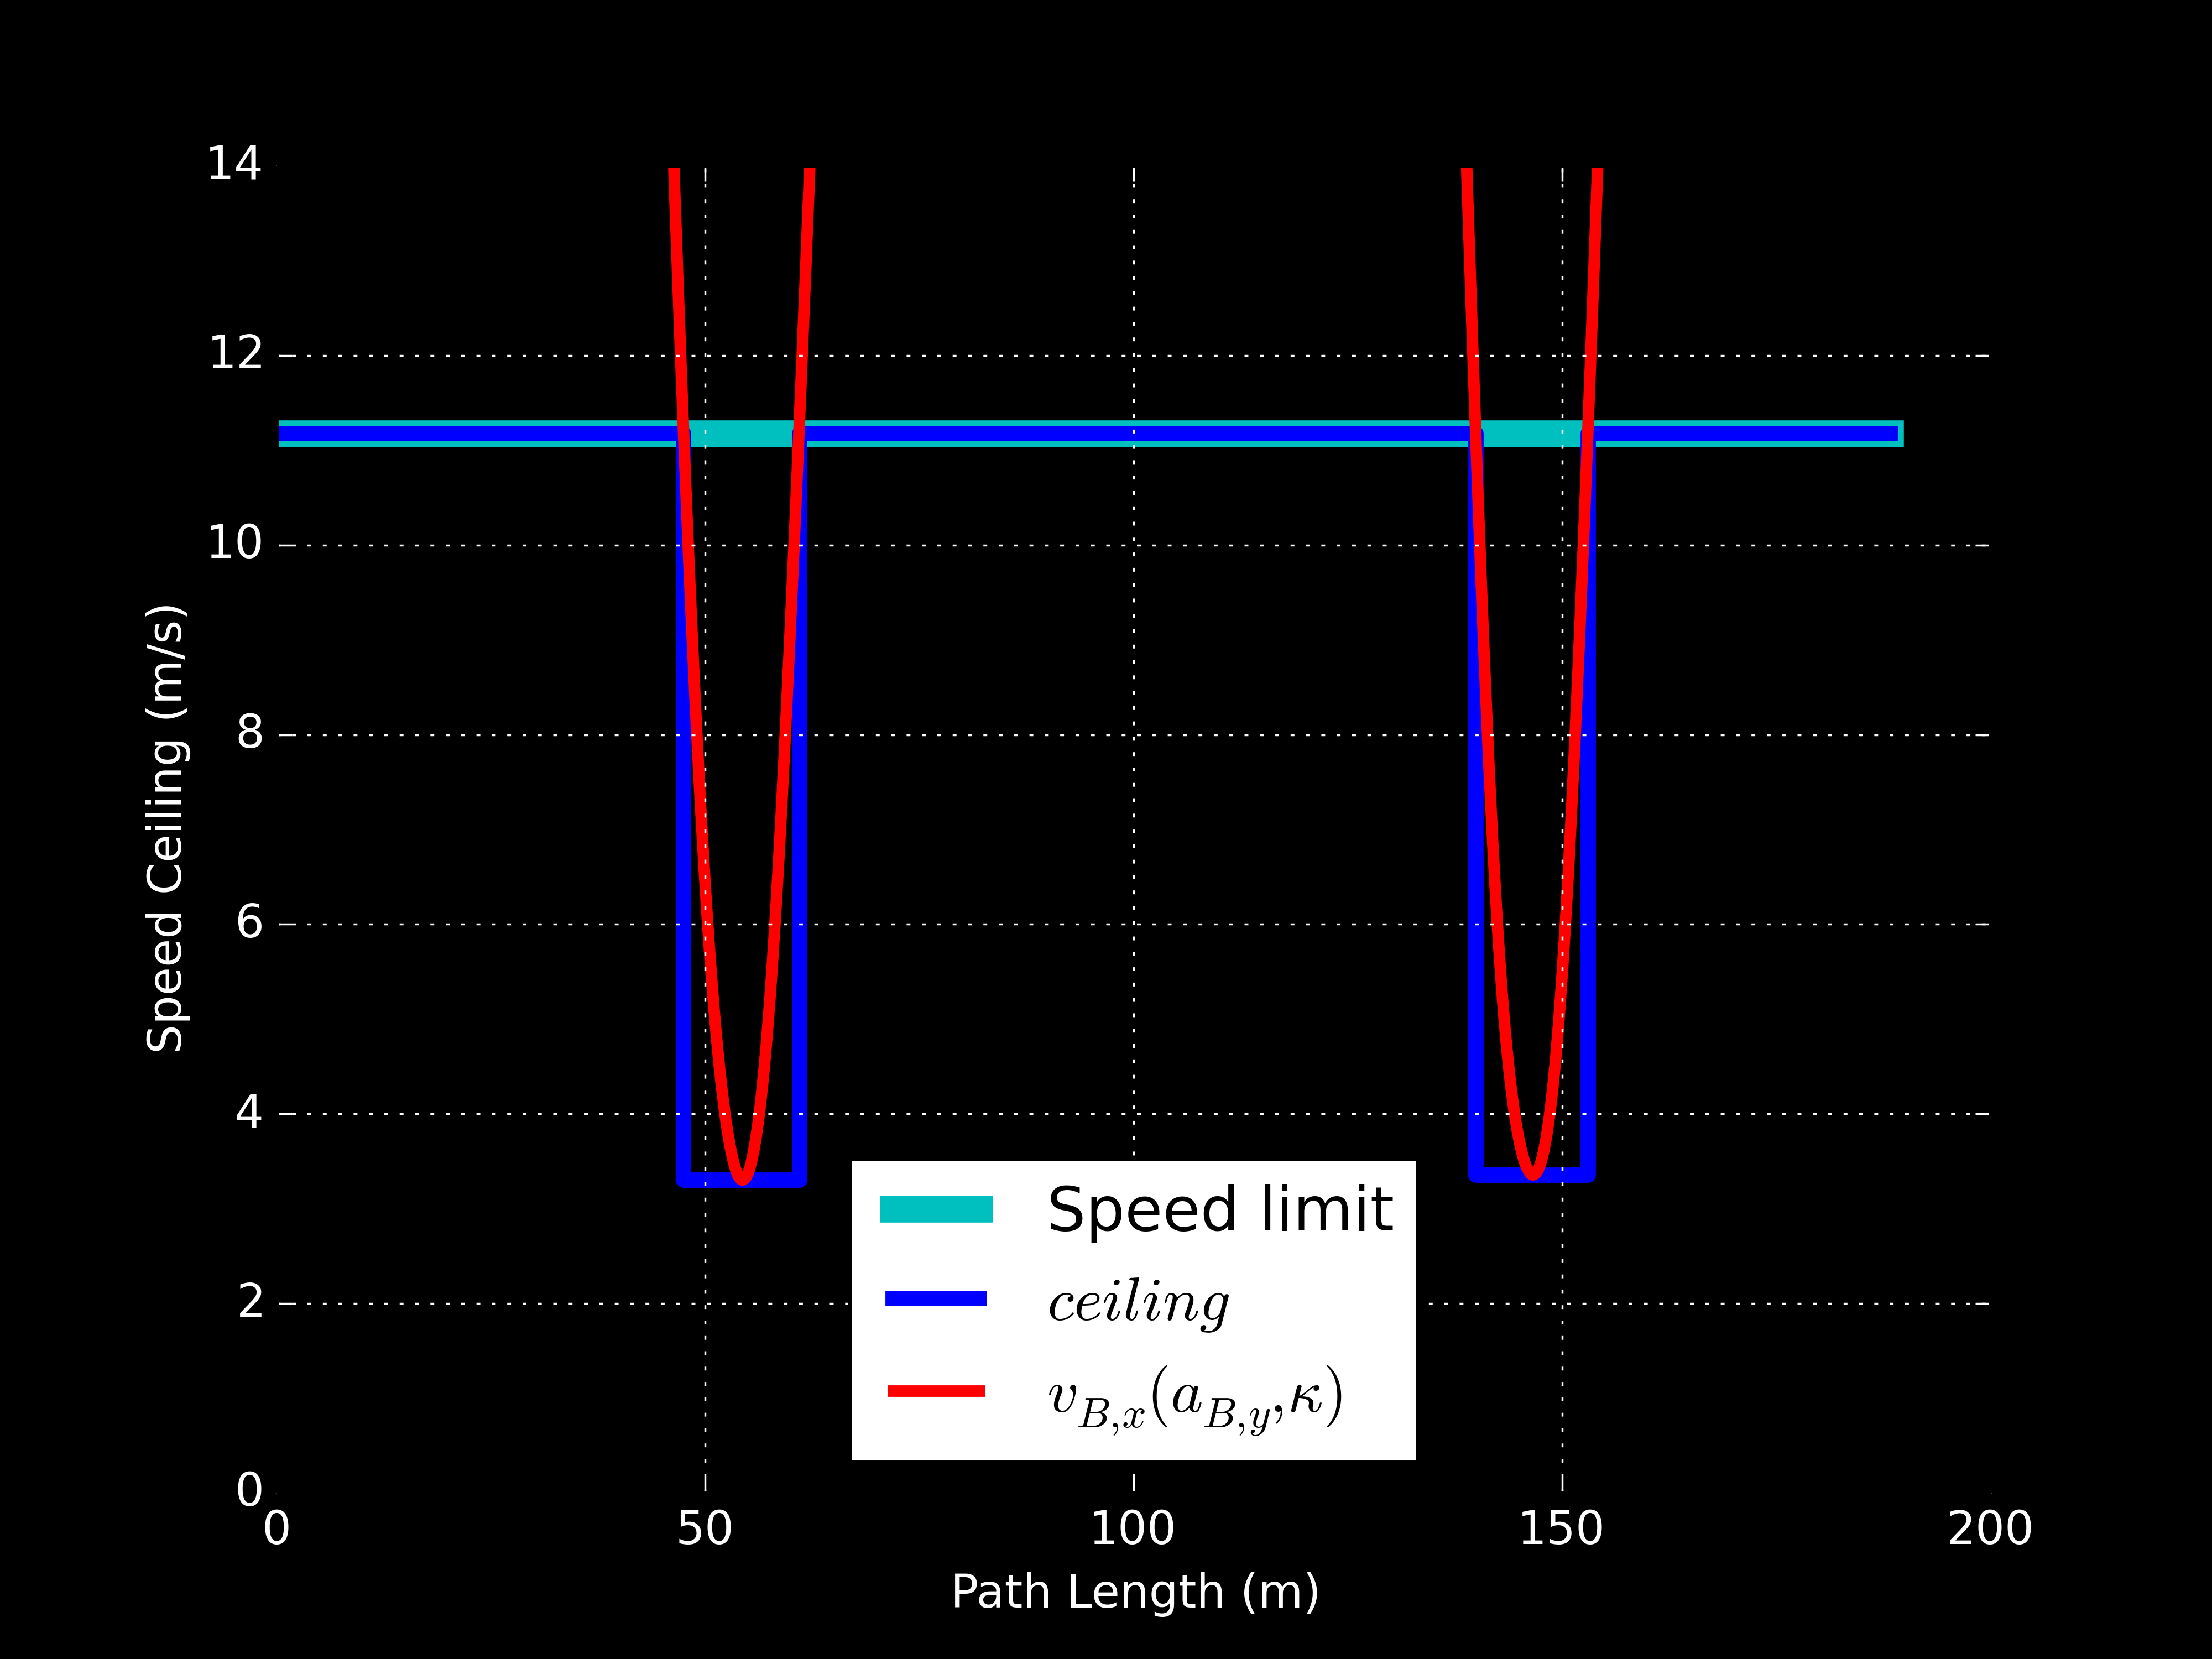
\includegraphics[width=0.5\columnwidth]{graphics/speed_ceiling.png}
  \caption{Speed Ceiling}
  \label{fig:speedceil}
\end{figure}

\begin{figure}[thpb]
  \centering
  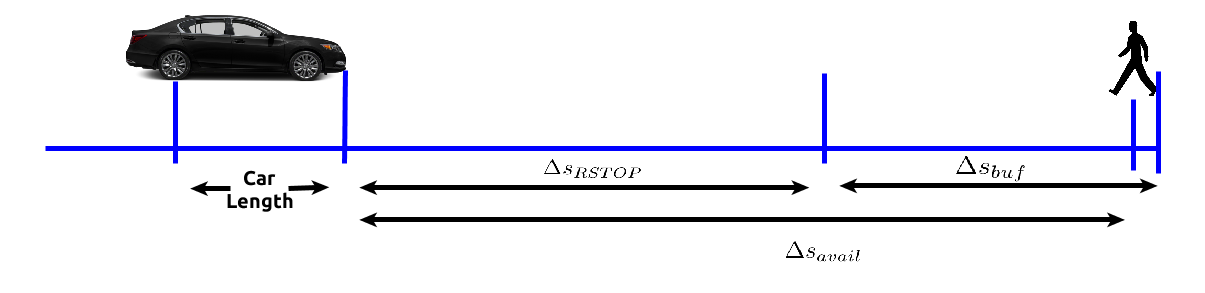
\includegraphics[width=1.0\columnwidth]{graphics/RSTOP_NORMAL_time_to_stop.png}
  \caption{Reaction Response: Normal Mode}
  \label{fig:7phaseprofile}
\end{figure}

%%%%%%%%%%%%%%%%%%%%%%%%%%%%%%%%%%%%%%%%%%%%%%%%%%%%%%%%%%%%%%%%%%%%%%%%%%%%%%%%
%%%%%%%%%%%%%%%%%%%%%%%%%%%%%%%%%%%%%%%%%%%%%%%%%%%%%%%%%%%%%%%%%%%%%%%%%%%%%%%%

\section{Implementation}

\emph{How much should we say here?}

%%%%%%%%%%%%%%%%%%%%%%%%%%%%%%%%%%%%%%%%%%%%%%%%%%%%%%%%%%%%%%%%%%%%%%%%%%%%%%%%
%%%%%%%%%%%%%%%%%%%%%%%%%%%%%%%%%%%%%%%%%%%%%%%%%%%%%%%%%%%%%%%%%%%%%%%%%%%%%%%%

\section*{Acknowledgments}

Thanks...

%%%%%%%%%%%%%%%%%%%%%%%%%%%%%%%%%%%%%%%%%%%%%%%%%%%%%%%%%%%%%%%%%%%%%%%%%%%%%%%%
%%%%%%%%%%%%%%%%%%%%%%%%%%%%%%%%%%%%%%%%%%%%%%%%%%%%%%%%%%%%%%%%%%%%%%%%%%%%%%%%
%%%%%%%%%%%%%%%%%%%%%%%%%%%%%%%%%%%%%%%%%%%%%%%%%%%%%%%%%%%%%%%%%%%%%%%%%%%%%%%%

\bibliographystyle{IEEEtran}
\bibliography{HRI_internship_trajectory_planner_articles}

\end{document}